\documentclass[12pt,a4paper,openany,final,twoside,longbibliography,hidelinks]{book}
\usepackage{acronym}
\usepackage[english]{babel}
\usepackage[utf8]{inputenc}
\usepackage[T1]{fontenc}
\usepackage{amsmath}
\usepackage{mathtools}
\usepackage{amsfonts}
\usepackage{amssymb}
\usepackage{bbold}
\usepackage{esdiff}
\usepackage[]{graphicx}
\usepackage[sort&compress,numbers]{natbib}
\bibliographystyle{aipnum4-2}
\usepackage{doi}
\renewcommand*{\bibfont}{\interlinepenalty 10000\relax}
\usepackage[defaultlines=2,all]{nowidow}
\usepackage{siunitx}
\sisetup{range-phrase=--}
\sisetup{range-units=single}

\usepackage[dvipsnames]{xcolor}
\usepackage{bm}
\usepackage{float}
\usepackage{verbatim}
\usepackage{afterpage}
\usepackage{microtype}
\usepackage[labelfont=bf]{caption}
\captionsetup[table]{position=above}
\usepackage{subfigure} 
\usepackage[onehalfspacing]{setspace}
\usepackage{blindtext} 
\numberwithin{equation}{section}
\usepackage{etoolbox}
\graphicspath{{./images/}}
\usepackage[]{geometry}
\usepackage[nottoc,notlof]{tocbibind}
\usepackage[ddmmyyyy]{datetime}
\renewcommand{\dateseparator}{.}

\usepackage{fancyhdr} 

\pagestyle{fancy}
\renewcommand{\chaptermark}[1]{\markboth{\thechapter.\space#1}{}} 

\fancypagestyle{schluss}{
    \fancyhead{}
    \fancyfoot[EL]{\thepage} 
    \fancyfoot[OR]{\thepage}
    \renewcommand{\headrulewidth}{0pt}}\graphicspath{{./images/}}
    
\fancyhf{}  % Kopf- und Fußzeile leeren 
\makeatletter
\let\ps@plain\ps@fancy
\makeatother

\fancypagestyle{myfancy}{
\newcommand{\lmod}{\fontfamily{lmodern}\fontsize{9}{11}\selectfont}
\fancyhead[EL,OL]{\lmod \nouppercase{\scshape\leftmark}} 
\fancyhead[ER,OR]{\lmod \nouppercase{\scshape\rightmark}} 
\fancyfoot[EL]{\lmod\thepage} 
\fancyfoot[OR]{\lmod\thepage}} 
\renewcommand{\chaptermark}[1]{\markboth{\thechapter.\space#1}{}} 


\fancypagestyle{schluss}{
    \fancyhead{}
    \fancyfoot[EL]{\thepage} 
    \fancyfoot[OR]{\thepage}
    \renewcommand{\headrulewidth}{0pt}}
\fancyhf{} 




\newcommand{\sg}[1]{\textcolor{blue}{#1}}
\newcommand{\ui}[1]{\textcolor{Green}{#1}}

\DeclareMathOperator{\Tr}{Tr}
\newcommand{\red}[1]{\textcolor{red}{#1}}
\newcommand{\wert}[3]{\SI[separate-uncertainty=true]{#1(#2)}{#3}}
\newcommand{\abs}[1]{\ensuremath{\left\vert#1\right\vert}}
\newcommand{\ket}[1]{\ensuremath{\left\vert #1\right>}}
\newcommand{\bra}[1]{\ensuremath{\left<#1\right\vert}}
\newcommand{\kasten}[1]{\mbox{\color{#1}$\blacksquare$}}
\newcommand{\rgbbox}[1]{\mbox{\color[RGB]{#1}$\blacksquare$}}
\newcommand{\hexbox}[1]{\mbox{\color[HTML]{#1}$\blacksquare$}}
\newcommand{\dint}[1]{\ensuremath{\mathop{\mathrm{d}#1}}}
\newcommand{\vect}[1]{\mathbf{#1}}


\usepackage{lmodern}
\makeatletter
\patchcmd{\BR@backref}{\newblock}{\newblock(\mbox{on thesis page}~}{}{}
\patchcmd{\BR@backref}{\par}{)\par}{}{}
\makeatother




\begin{document}

\pagenumbering{gobble}

\begin{titlepage}
    \begin{center}
	{\scshape\Large Dissertation\\}
	\vspace{.1cm}
	\rule[1pt]{\textwidth}{1.5pt}
    \LARGE{\textbf{Automated optimization of sensitivity in a search for boosted VBF Higgs pair production in the $b\overline{b}b\overline{b}$ quark final state with the ATLAS detector
	}}
    \rule[11pt]{\textwidth}{1.5pt}
	
    {\normalsize\textbf{For the attainment of the academic degree doctor rerum naturalium (Dr. rer. nat.) in the subject: Physics}} 
    \vspace{1cm}

    \Large{\textbf{M.Sc. Frederic Renner\\}}
	Berlin, \today\\
    \vspace{1cm}
    \large
	Faculty of Mathematics and Natural Sciences of the Humboldt University of Berlin\\
    \vspace{1cm}

	1st Supervisor: Dr. Clara Elisabeth Leitgeb\\
	2nd Supervisor: Prof. Dr. Cigdem Issever
	\vspace{01cm}


	\newpage 
	(Only after the disputation for publication in the university library according to § 15	of the doctoral regulations enter the names and the date):\\
	\raggedright
	Reviewers: \\
	1st: \\
	2nd: \\
	3rd: \\
	
	Date of the oral examination: 
\end{center}
\end{titlepage}

\newpage 
\quad
\thispagestyle{empty}

\newpage 
\thispagestyle{empty}
\begin{center}
    \textbf{Abstract}
\end{center}
%\vspace{.5cm}
\noindent I am an abstract.

\newpage
\quad
\thispagestyle{empty}
\tableofcontents

\newpage
\thispagestyle{empty}
\listoffigures


\newpage
\quad
% \thispagestyle{empty}



\newpage 
\thispagestyle{empty}
\quad  

\newpage
\thispagestyle{empty}
\pagestyle{myfancy}
\pagenumbering{arabic}


%-------------------------------------------------------------


% \chapter{Introduction}


https://arxiv.org/pdf/2207.00043.pdf

mehr gründe warum physik versteckt in top und higgs präziosions messungen... 
\chapter{Theory}
\noindent The \ac{sm} of Particle Physics is the current theory that describes three of the four fundamental forces, namely the electromagnetic, strong, and weak forces, with the exception of gravity. Over the last decades it has been probed with remarkable precision but although there are  observational phenomena that lie beyond its scope.

The SM is based on symmetry principles and is described by a lorentz-invariant \ac{qft} that is renormalizable and invariant under local gauge transformations. This means that within the non-abelian gauge group
\begin{equation}
    G = SU(3)_C \otimes SU(2)_L \otimes U(1)_Y,
\end{equation}
the equations of motions are invariant. $SU(3)_C$ is the special unitary group of rank 3 representing the color symmetry within \ac{qcd}, the \ac{qft} describing the strong interactions. $SU(2)_L \otimes U(1)_Y$ exhibits the unification of the weak and electromagnetic interaction into the electro-weak force of $SU(2)_L$ left-chiral fermions of the weak force and right-handed $U(1)_Y$ fermions with hypercharge $Y$ of the electromagnetic force described by Quantum Electrodynamics \ac{qed}.

The following describes the particles of the \ac{sm} and gives a brief overview of the \ac{qft}'s used to describe aforementioned forces. The content of this chapter draws inspiration primarily from \citep{hollik2010quantum,griffiths2020introduction,thomson2013modern,zee2010quantum}. Natural units are assumed everywhere $\hbar=c=1$.


\section{Particles of the Standard Model}

All currently known elementary particles are included in the \ac{sm} and can be organized as depicted in figure \ref{fig:sm}. This includes 12 fermions, that are particles of half-integer spin, 12 vector bosons with spin 1, and the Higgs boson, a scalar particle with spin 0.


\begin{figure}
    \centering
    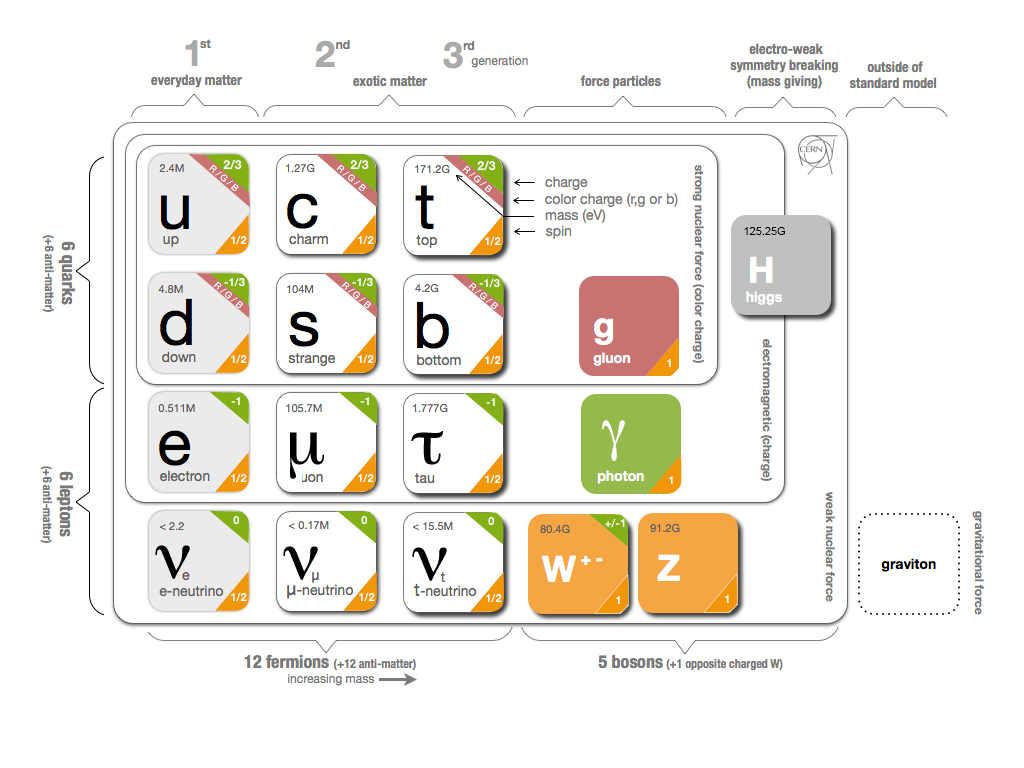
\includegraphics[width=1\textwidth]{SMinfographic_image_}
    \caption[]{Particles in the SM. Adopted from \citep{smpar}. Higgs Boson mass corrected to the current value \citep{particle2022review}. }
    \label{fig:sm}
\end{figure}


The fermions can be categorized into three generations each consisting of a charged lepton, a neutral neutrino and two quarks. Except for their masses, particles of the different generations have the same quantum numbers. Ordinary matter consists only of particles from the first generation. Moreover each particle has an associated anti-particle with all the quantum numbers inversed.

Quarks possess both electric charges and color charges, causing them to interact with each other via weak, electromagnetic, and strong forces. Each generation consists of an up quark (up, charm and top quark) with an electric charge of \mbox{Q = 2/3} and a down quark (down, strange and bottom quark) with a charge of \mbox{Q = -1/3}. Quarks can only be observed as composite particles - hadrons due to color confinement. This states that if one tries to separate a hadron, it is always energetically favorable to produce a quark-antiquark pair instead. Hadrons constitutes either bound states of 2 quarks - Mesons, e.g. a pion or 3 quarks - Baryons e.g. the proton. To not break Pauli's exclusion principle quarks in a bound state must have different color states.

Leptons in turn do not carry a color charge and encompasses the electron $e$, muon $\mu$ and tau $\tau$ and their associated neutrinos $\nu_e$, $\nu_\mu$ and $\nu_\tau$. In the \ac{sm} neutrinos are considered to be massless. Neutrinos also do not carry a charge and interact solely via the weak force whereas the  ones ($e$, $\mu$, $\tau$) with a charge $Q=-1$ participate also interact electromagnetically.

In the interaction picture of \ac{qft}, forces are mediated by particles specific to the particular force. These particles are bosons and are mediating as 8 massless gluons $g$ the strong force, as 1 massless photon $\gamma$ the electromagnetic force and as 3 massive bosons $W^+,W^-,Z$ the weak force.

The scalar Higgs particle has a unique role in the Standard model. A locally gauge invariant \ac{qft} requires massless mediators which the $W^{\pm},Z$ are not. When unifying the weak force and the electromagnetic force into the electroweak force a new field - the Higgs field - can incorporate mass to these mediators by leaving the qft gauge invariant. This will be discussed in detail in section \ref{sec:higgs_mechanism}. The Higgs field can explain the masses of all fermions as the coupling to each fermion is proportional to its mass. This essentially means that the heavier the particle, the stronger its interaction is with the Higgs field.

If not further specified the following always includes the anti-particles when referred to a species or a particular particle.

\section{Quantum Field Theory}\label{sec:qft}
Elementary Particles can be created, transformed and vanish in all sorts of particle interactions. Quantum mechanics states that energy can vary greatly on short time scales via the uncertainty principle. Special relativity relates energy with mass allowing energy to manifest as massive particles. Though special relativity lacks a quantum mechanical description and in non-relativistic quantum mechanics the particle number is conserved. Neither of these descriptions is sufficient to fully describe the observations therefore \ac{qft} was developed.

For a field description some quantity $\phi(x,y,z,t)=\phi(x)$ is assigned to some region in spacetime $x$. Similar to the Lagrangian formalism in classical mechanics here a Lagrangian density in spacetime governs the dynamics of the system $\mathcal{L}(\phi_1,\dots,\phi_n)$. The generalized Euler-Lagrange equations of qft then give the according equations of motion for each field component $\phi_i$
\begin{equation}
    \partial_\mu \left(\frac{\partial\mathcal{L}}{\partial(\partial_\mu\phi_i)}\right)=\frac{\partial\mathcal{L}}{\partial \phi_i}.
\end{equation}
This relation gives the equations of motion for the Lagrangian. Fields which appear in the \ac{sm} and their associated Lagrangian are summarized in \ref{tab:fields} table.
\begin{table}
    \begin{center}
        \begin{tabular}{c|c|c}
            particle           & field type      & Lagrange                                                                                                     \\ [1ex]  \hline
            spin-0 (scalar)    & scalar $\phi$   & $\mathcal{L}_\mathrm{Klein-Gordon}=\frac{1}{2} (\partial_\mu \phi )(\partial^\mu \phi)-\frac{m^2}{2}\phi^2 $ \\  [1.5ex]
            spin-1/2 (fermion) & spinor $\psi$   & $\mathcal{L}_\mathrm{Dirac}= \overline{\psi}(i \gamma^\mu \partial_\mu - m )\psi$                            \\  [1.5ex]
            spin-1 (boson)     & vector  $A_\mu$ & $\mathcal{L}_\mathrm{Proca}= -\frac{1}{4}F_{\mu\nu}F^{\mu\nu} +\frac{m^2}{2} A_\mu A^\mu$                    \\  [2ex]
        \end{tabular}
        \caption{Quantum fields relevant for the \ac{sm}. With $F_{\mu\nu}=\partial_\mu A_\nu - \partial_\nu A_\mu$ the electromagnetic field strength tensor.}
        \label{tab:fields}
    \end{center}
\end{table}

In \ac{qft} the conventional strategy to describe particle dynamics is to use a perturbation ansatz $\mathcal{L}=\mathcal{L}_0+\mathcal{L}_1$ where one knows the solution of $\mathcal{L}_0$ and adds a small perturbation $\mathcal{L}_1$. Herein the free field/kinetic part of the Lagrangian is \mbox{$\mathcal{L}_0=\frac{1}{2}[(\partial_\mu \phi)^2 - m^2\phi^2] $} and a small perturbation/potential term $\mathcal{L}_1=V(\phi)$ is added as some polyominal in $\phi$ that governs the interactions of particles. A term $J(x)\phi(x)$ needs to be added to excite the field or create/destroy particles so that the ansatz reads
\begin{equation}
    \mathcal{L}=\frac{1}{2}[(\partial_\mu \phi)^2 - m^2\phi^2]
    -V(\phi) + J(x)\phi(x).
\end{equation}
In the path integral formulation of \ac{qft} the problem can be reduced to integrals of the form \mbox{$\int D\phi e^{i\int d^4x \mathcal{L}(\phi(\bm{x},t))}$}. Where $\int D\phi$ is the integral over all possible paths of the field. Usually $V(\phi)$ is just one anharmonic term with $\lambda\phi^4$ with coupling strength $\lambda$ and is expanded in $e$ to make the integral solvable
\begin{equation}
    e^{-V(\phi)}=e^{-\lambda\phi^4}=1-\lambda\phi^4+\frac{1}{2}\lambda^2\phi^8+\dots
\end{equation}
This only works if $\lambda$ is small. The result is a probability also called the amplitude usually denoted with $\mathcal{M}$. Via this one can derive the Feynman rules and calculate cross sections to a desired order of expansion.

The principle of local gauge invariance generates all the symmetries for the different forces and is inspired by gauge invariance from classical electrodynamics. In the following, this is explained for each of the forces.

\section{Quantum Electrodynamics}\label{sec:qed}
The \ac{qft}-description of the electromagnetic interaction \ac{qed} can be derived from the free fermion field given by the Dirac equation
\begin{equation}
    \mathcal{L}_\mathrm{Dirac} = \overline{\psi}(i \gamma^\mu \partial_\mu - m )\psi.
    \label{eq:dirac}
\end{equation}
This Lagrangian is invariant under a change of phase $\alpha$
\begin{equation}
    \psi(x) \rightarrow  e^{-i \alpha}\psi(x).
\end{equation}
The requirement that this transformation also holds locally means that $\alpha$ now additionally depends on the point $x$ in spacetime $\alpha \rightarrow \alpha(x)$. Since this gives another term because of the derivative, the Lagrangian can be made invariant again by introducing a vector field $A_\mu$ with a coupling of the size of the electron charge $e$ and replacing the derivative $\partial_\mu$ by the covariant derivative $D_\mu$
\begin{equation}
    \partial_\mu \rightarrow D_\mu = \partial_\mu + ie A_\mu.
    \label{eq:cov_diff}
\end{equation}
Thus, the new Lagrangian
\begin{equation}
    \mathcal{L} = \overline{\psi}(i \gamma^\mu D_\mu - m )\psi
    =
    \underbrace{\overline{\psi}(i \gamma^\mu \partial_\mu - m )\psi}_{\mathcal{L}_\mathrm{Dirac} }
    +
    \underbrace{ e\overline{\psi} \gamma^\mu {\psi}A_\mu}_{\mathcal{L}_\mathrm{int}}
\end{equation}
becomes invariant under the local gauge transformations
\begin{align}
    \psi(x)  & \rightarrow  e^{-i \alpha(x)}\psi(x)                      \\
    A_\mu(x) & \xrightarrow{} A_\mu(x) -\frac{1}{e}\partial_\mu\alpha(x)
\end{align}
forming the electromagnetic $U(1)_{EM}$ gauge group. This is also called the minimal substitution rule. This Lagrangian describes a fermion interacting with a vector field $A_\mu$ - the photon. A kinetic term for the vector field can be from the Proca Lagrangian in table \ref{tab:fields}. $F_{\mu\nu}$ is local gauge invariant whereas the $A_\mu A^\mu$ is not, which is why the gauge field is required to be massless. The full \ac{qed} lagrangian with coupling strength  then
\begin{equation}
    \mathcal{L}_\mathrm{QED}
    =
    \underbrace{\overline{\psi}(i \gamma^\mu \partial_\mu - m )\psi}_{\mathcal{L}_\mathrm{Dirac} }
    +
    \underbrace{ e\overline{\psi} \gamma^\mu {\psi}A_\mu}_{\mathcal{L}_\mathrm{int}}
    -
    \underbrace{\frac{1}{4}F_{\mu\nu}F^{\mu\nu}}_{\mathcal{L}_\mathrm{Maxwell} }.
    \label{eq:l_qed}
\end{equation}
Saying that this symmetry for $\alpha(x)$ holds locally for all unitary $1\times1$  matrices $U(1)$ is a bit extravagant, but the formalism is extendable to higher orders as for the electroweak theory and \ac{qcd} case. It is called an abelian gauge group as any $1\times1$ matrix also commutes with itself.

\section{Quantum Chromodynamics}

Along the same lines as \ac{qed} is derived in section \ref{sec:qed}, the theory of the strong interactions \ac{qcd} is now a non-abelian gauge theory of the symmetry group $SU(3)$. The latter is generated by the $3\times 3$ Gellmann matrices $\lambda_a$ with $ a\in\{1,\mathellipsis,8\}$. The fundamental charge is now color and each quark is a triplet of the three color fermion fields $\Psi_k=(\psi_r,\psi_g,\psi_b)^T$ for all quark flavors $k$. Local gauge invariance of the Lagrangian
\begin{equation}
    \mathcal{L} =
    \sum_k
    \begin{pmatrix}
        \overline{\psi}_r & \overline{\psi}_g & \overline{\psi}_b
    \end{pmatrix}
    (i \gamma^\mu \partial_\mu - m )
    \begin{pmatrix}
        \psi_r \\
        \psi_g \\
        \psi_b
    \end{pmatrix}
    =
    \sum_k
    \overline{\Psi}_k(i \gamma^\mu \partial_\mu - m )\Psi_k
    \label{eq:dirac}
\end{equation}
can be achieved via the gauge transformations of the spinors
\begin{equation}
    \Psi_k(x) \rightarrow e^{i \alpha_a(x) \lambda_a/2} \Psi_k(x),\qquad \alpha\in\mathbb{R},\quad a\in\{1,\mathellipsis,8\},
\end{equation}
with $\alpha_a(x)$ a local phase and the index $a$ for the 8 gluons. Here and in the following  summation over equal indices $\alpha_a(x) \lambda_a=\sum_i \alpha_a(x) \lambda_a$ is assumed. As in \ac{qed} a covariant derivative is introduced
\begin{equation}
    D_\mu = \partial_\mu - i g_s \frac{\lambda_a}{2}G_\mu^a,
\end{equation}
involving the eight gluon vector fields $G_\mu^a$ and the coupling strength $g_s$, which is related to the strong coupling constant as
\begin{equation}
    \alpha_s=\frac{g_s^2}{4\pi}.
\end{equation}
Again self coupling terms are added
\begin{equation}
    G^a_{\mu\nu}=\partial_\mu G_\nu^a-\partial_\nu G_\mu^a+g_s f^a_{\beta\gamma}G^\beta_\mu G_\nu^\gamma, \qquad \text{with } [\lambda_a,\lambda_b]= i f_{ab}^c \lambda_c,
\end{equation}
to get the gauge invariant \ac{qcd} Lagrangian
\begin{align}
    {\mathcal {L}}_{\text{QCD}} & =\sum_k\overline{\Psi}_k\left( i \gamma^\mu D_\mu-m_k\right)\Psi_k-{\frac {1}{4}}G_{\mu \nu }^{a}G^{a\mu \nu}                                                                                    \\
                                & =\sum_k{\overline{\Psi}_k}\left(i\gamma^\mu \partial_\mu-m_k\right)\Psi_k+ g_s{\overline{\Psi}_k}\gamma ^{\mu }\frac{ \lambda_a}{2} \Psi_k G_\mu^a - {\frac {1}{4}}G_{\mu \nu }^{a}G^{a\mu \nu}.
    \label{eq:l_qcd}
\end{align}
This Lagrange consists of a kinetic term for each quark, an interaction term of the quarks with the gluons and gluon-gluon interactions giving vertices shown in \ref{fig:qcd_vertices}. This becomes clear when $G^a_{\mu\nu}$ is squared and also leads to cubic and quartic terms for the fields.
\begin{figure}[H]
    \centering
    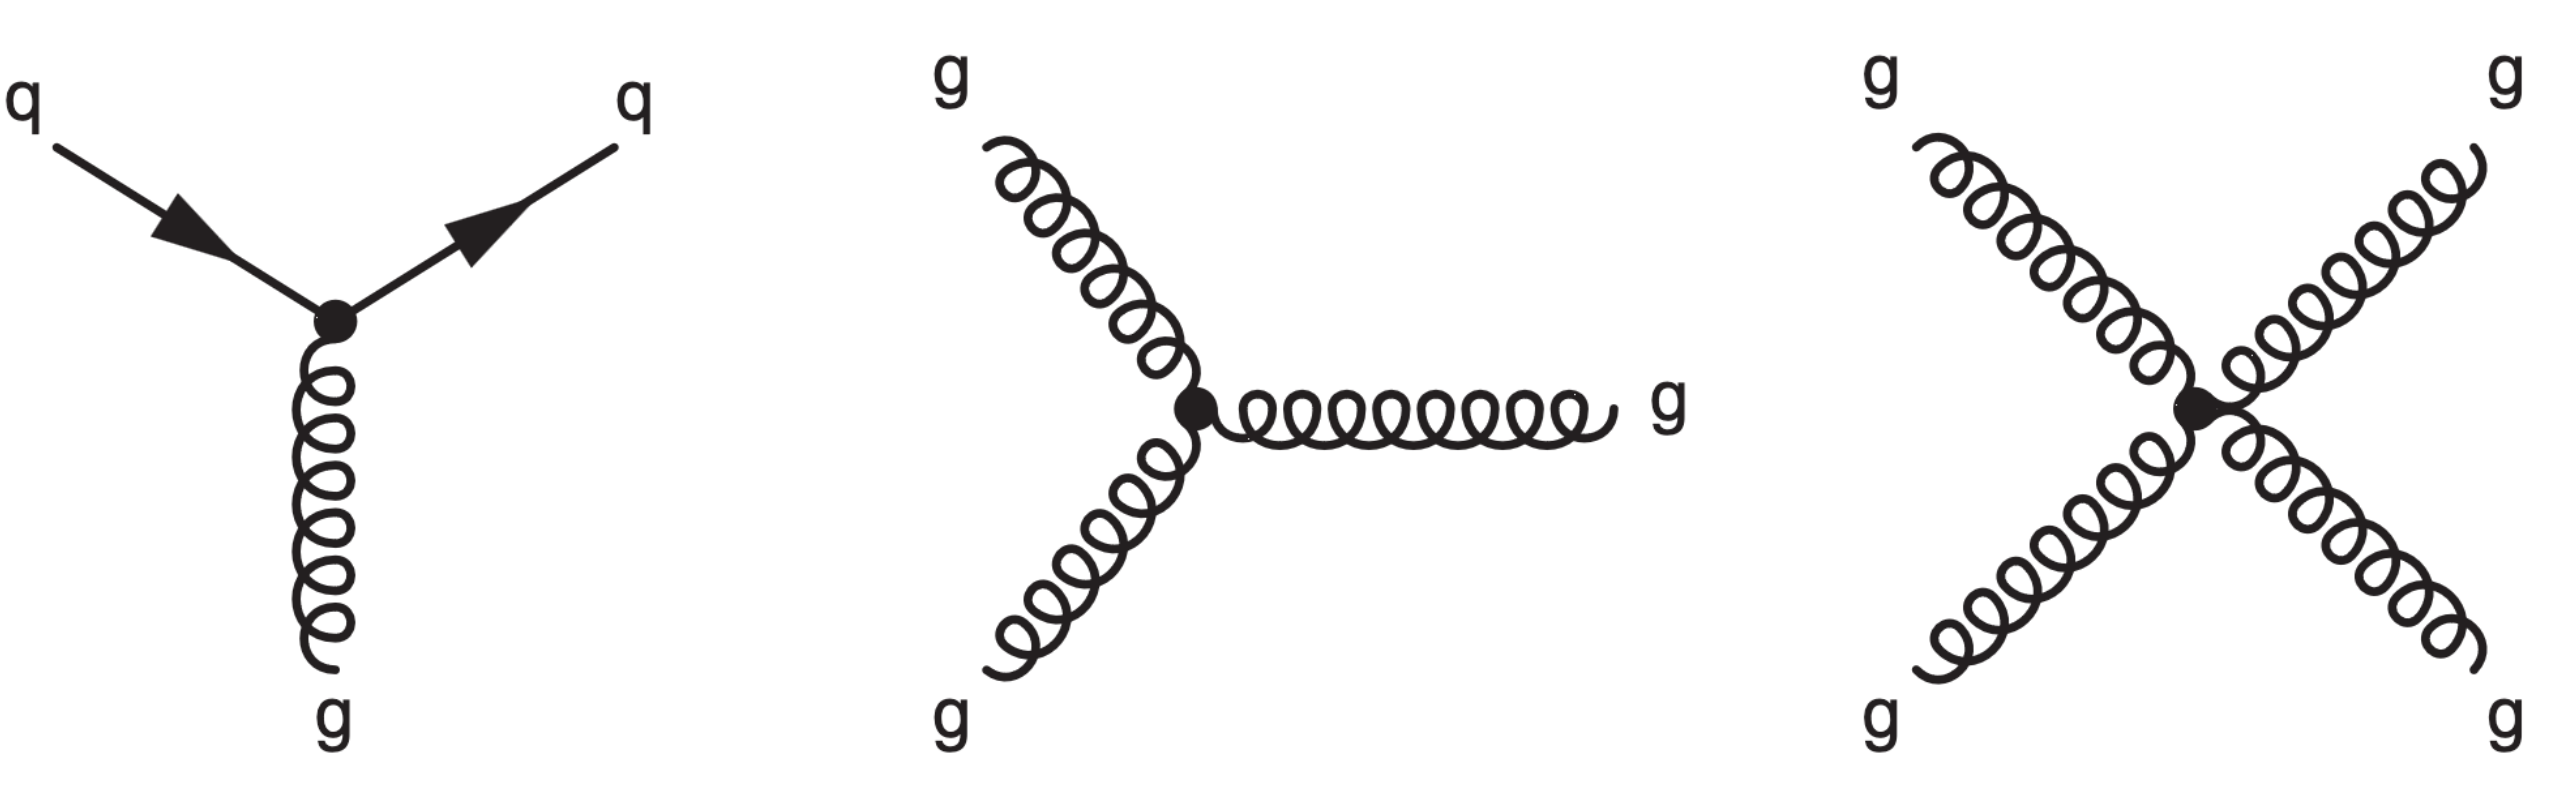
\includegraphics[width=0.8\textwidth]{gluon_gluon_interactions}
    \caption[]{(left) Quarks interacting with a gluon. (middle) triplet and (right) quartic self coupling of gluons. Adopted from \citep{thomson2013modern}.}
    \label{fig:qcd_vertices}
\end{figure}

\section{Renormalization}
\begin{figure}
    \centering
    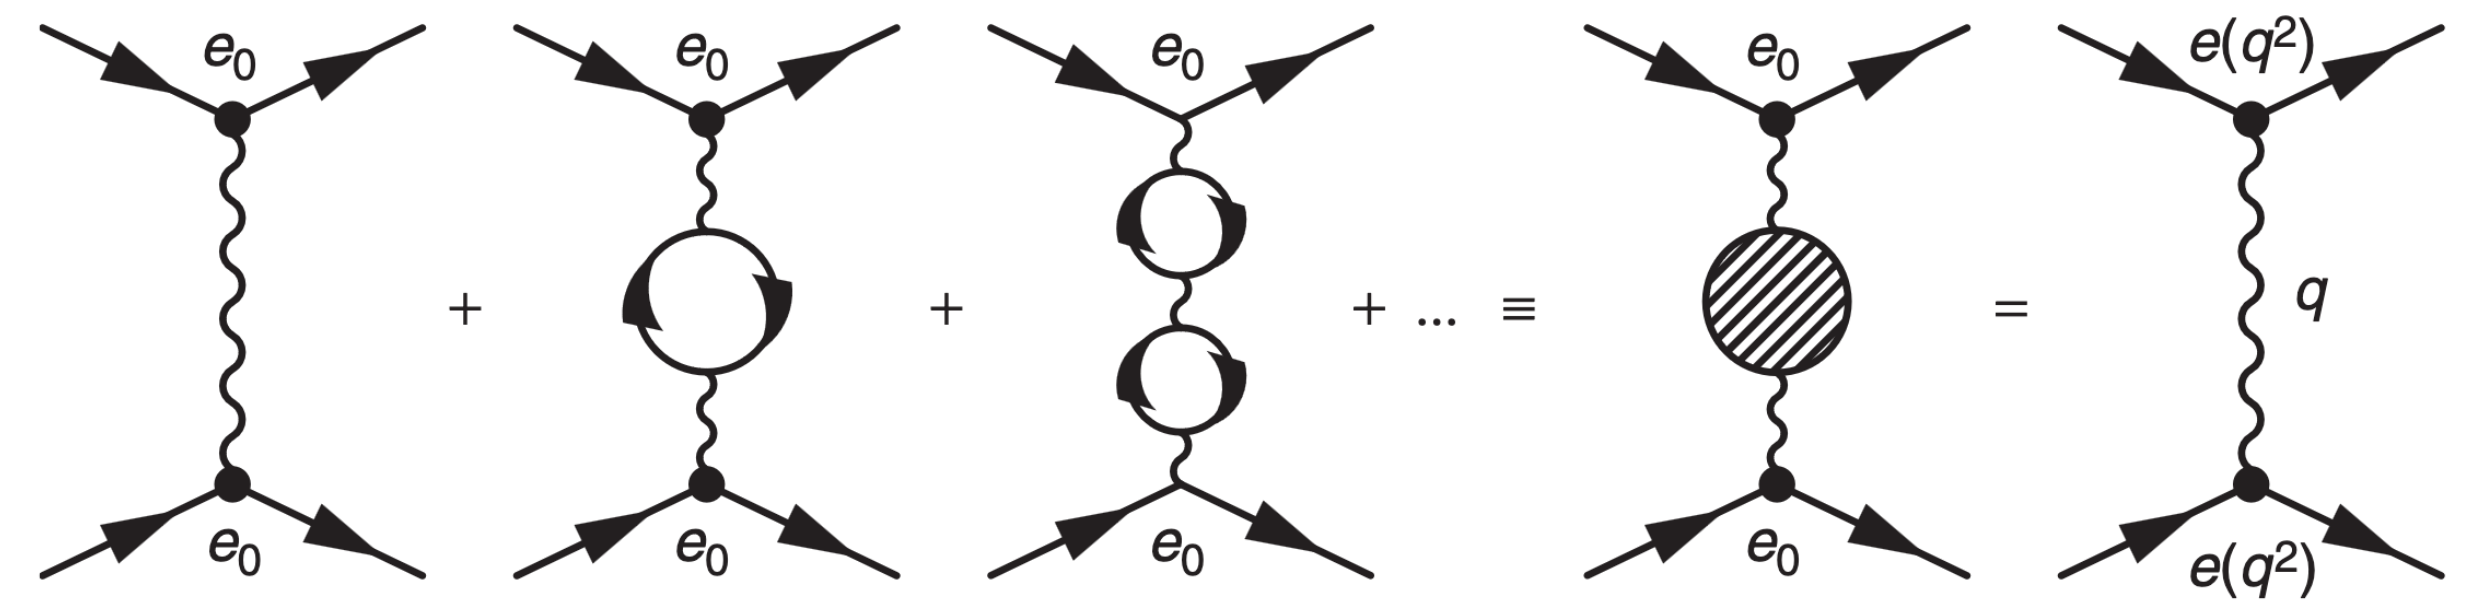
\includegraphics[width=1\textwidth]{qed_diagrams}
    \caption[]{Higher order loop corrections in \ac{qed} schematically treated as one effective diagram. Adopted from \citep{thomson2013modern}.}
    \label{fig:qed_diagrams}
\end{figure}
When trying to calculate amplitudes $\mathcal{M}$ of higher order diagrams in \ac{qed} like the second or third one in figure \ref{fig:qed_diagrams} it results in diverging integrals. These diagrams are also referred to as vacuum polarization as virtual particle-antiparticle pairs screen the actual charge of the electron $e_0$ like a dielectric medium in classical electrodynamics. The situation can be fixed by absorbing the appearing infinities into an effective charge/coupling $e(q^2)$ which is now a function of the squared four momentum $q^2$ at the virtual photon vertex shown schematically in figure \ref{fig:qed_diagrams}. For the the second diagram in figure \ref{fig:qed_diagrams} involving only one loop correction it can be shown that for some measured coupling $e(q^2=\mu^2)$ the actual coupling $e(q^2)$ follows a scaling behavior that holds if $q^2$ and $\mu^2$ are larger than the electron mass \citep{thomson2013modern}. The coupling constant is now a running coupling $e(q^2)$ and reads in terms of the fine structure constant $\alpha(q^2)=e^2(q^2)/4\pi$,
\begin{equation}
    \alpha(q^2)=
    \frac{\alpha(\mu^2)}
    {1-\alpha(\mu)\frac{1}{3\pi}
        \ln
        \left(\frac{q^2}{\mu^2}\right)}.
    \label{eq:qed_coupling}
\end{equation}
Therefore with increasing momentum transfer or closer approach in a collision the coupling at the virtual photon vertex increases as can be seen qualitatively in figure \ref{fig:renorm_scaling}(a).
\begin{figure}
    \centering
    \subfigure[]{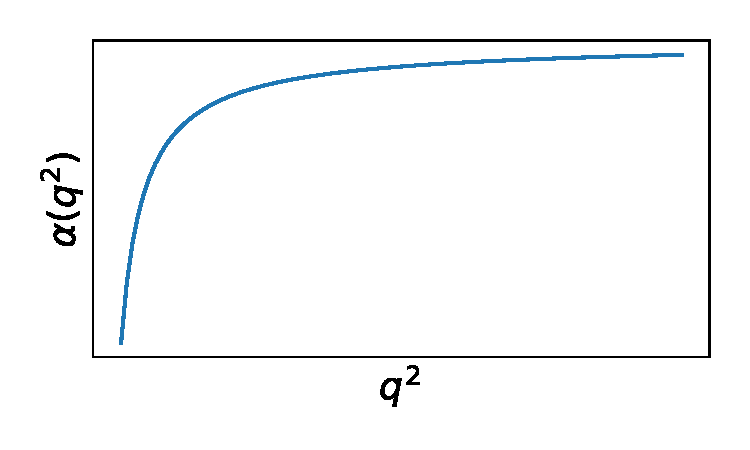
\includegraphics[width=.49\textwidth]{qed_scaling}}
    \subfigure[]{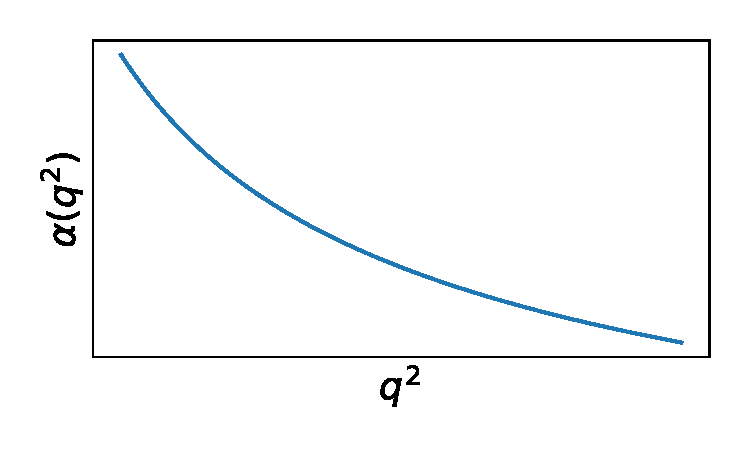
\includegraphics[width=.49\textwidth]{qcd_scaling}}
    \caption[]{Qualitative behavior of the running couplings for (\textbf{a}) \ac{qed} as of equation \ref{eq:qed_coupling} and (\textbf{b}) \ac{qcd} as of equation \ref{eq:qcd_coupling}.}
    \label{fig:renorm_scaling}
\end{figure}
\begin{figure}[H]
    \centering
    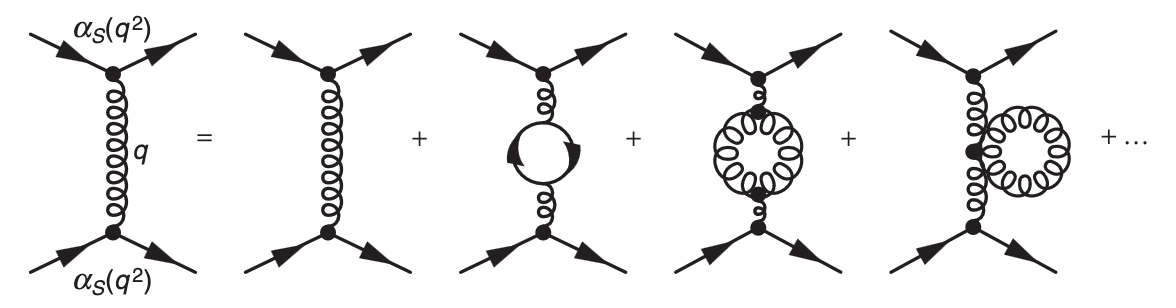
\includegraphics[width=1\textwidth]{qcd_diagrams}
    \caption[]{Some higher order loop corrections in \ac{qcd}. Adopted from \citep{thomson2013modern}.}
    \label{fig:qed_diagrams}
\end{figure}
Renormalization in \ac{qcd} can be derived similarly but also the quartic and triplet couplings exemplified in figure \ref{fig:qed_diagrams} need to be considered that result in a scaling for the strong coupling
\begin{equation}
    \alpha_S(q^2)=
    \frac{\alpha_S(\mu^2)}
    {1+B\alpha_S(\mu)
        \ln
        \left(\frac{q^2}{\mu^2}\right)}, \qquad \text{with } B=\frac{11N_c-2N_f}{12\pi}.
    \label{eq:qcd_coupling}
\end{equation}
For 3 color charges $N_c$ and 6 fermions $N_f$ in the \ac{sm}, $B$ is positive and the coupling becomes weaker for shorter scales or higher momentum transfer as can be seen in figure \ref{fig:renorm_scaling}(b).

The fine structure constant of \ac{qed} $\alpha(q^2\approx 0)\approx 1/137$ does not vary dramatically over the energy ranges of matter for particle physics as shown in figure \ref{fig:renorm_scaling_exp}(a).
\begin{figure}
    \centering
    \subfigure[]{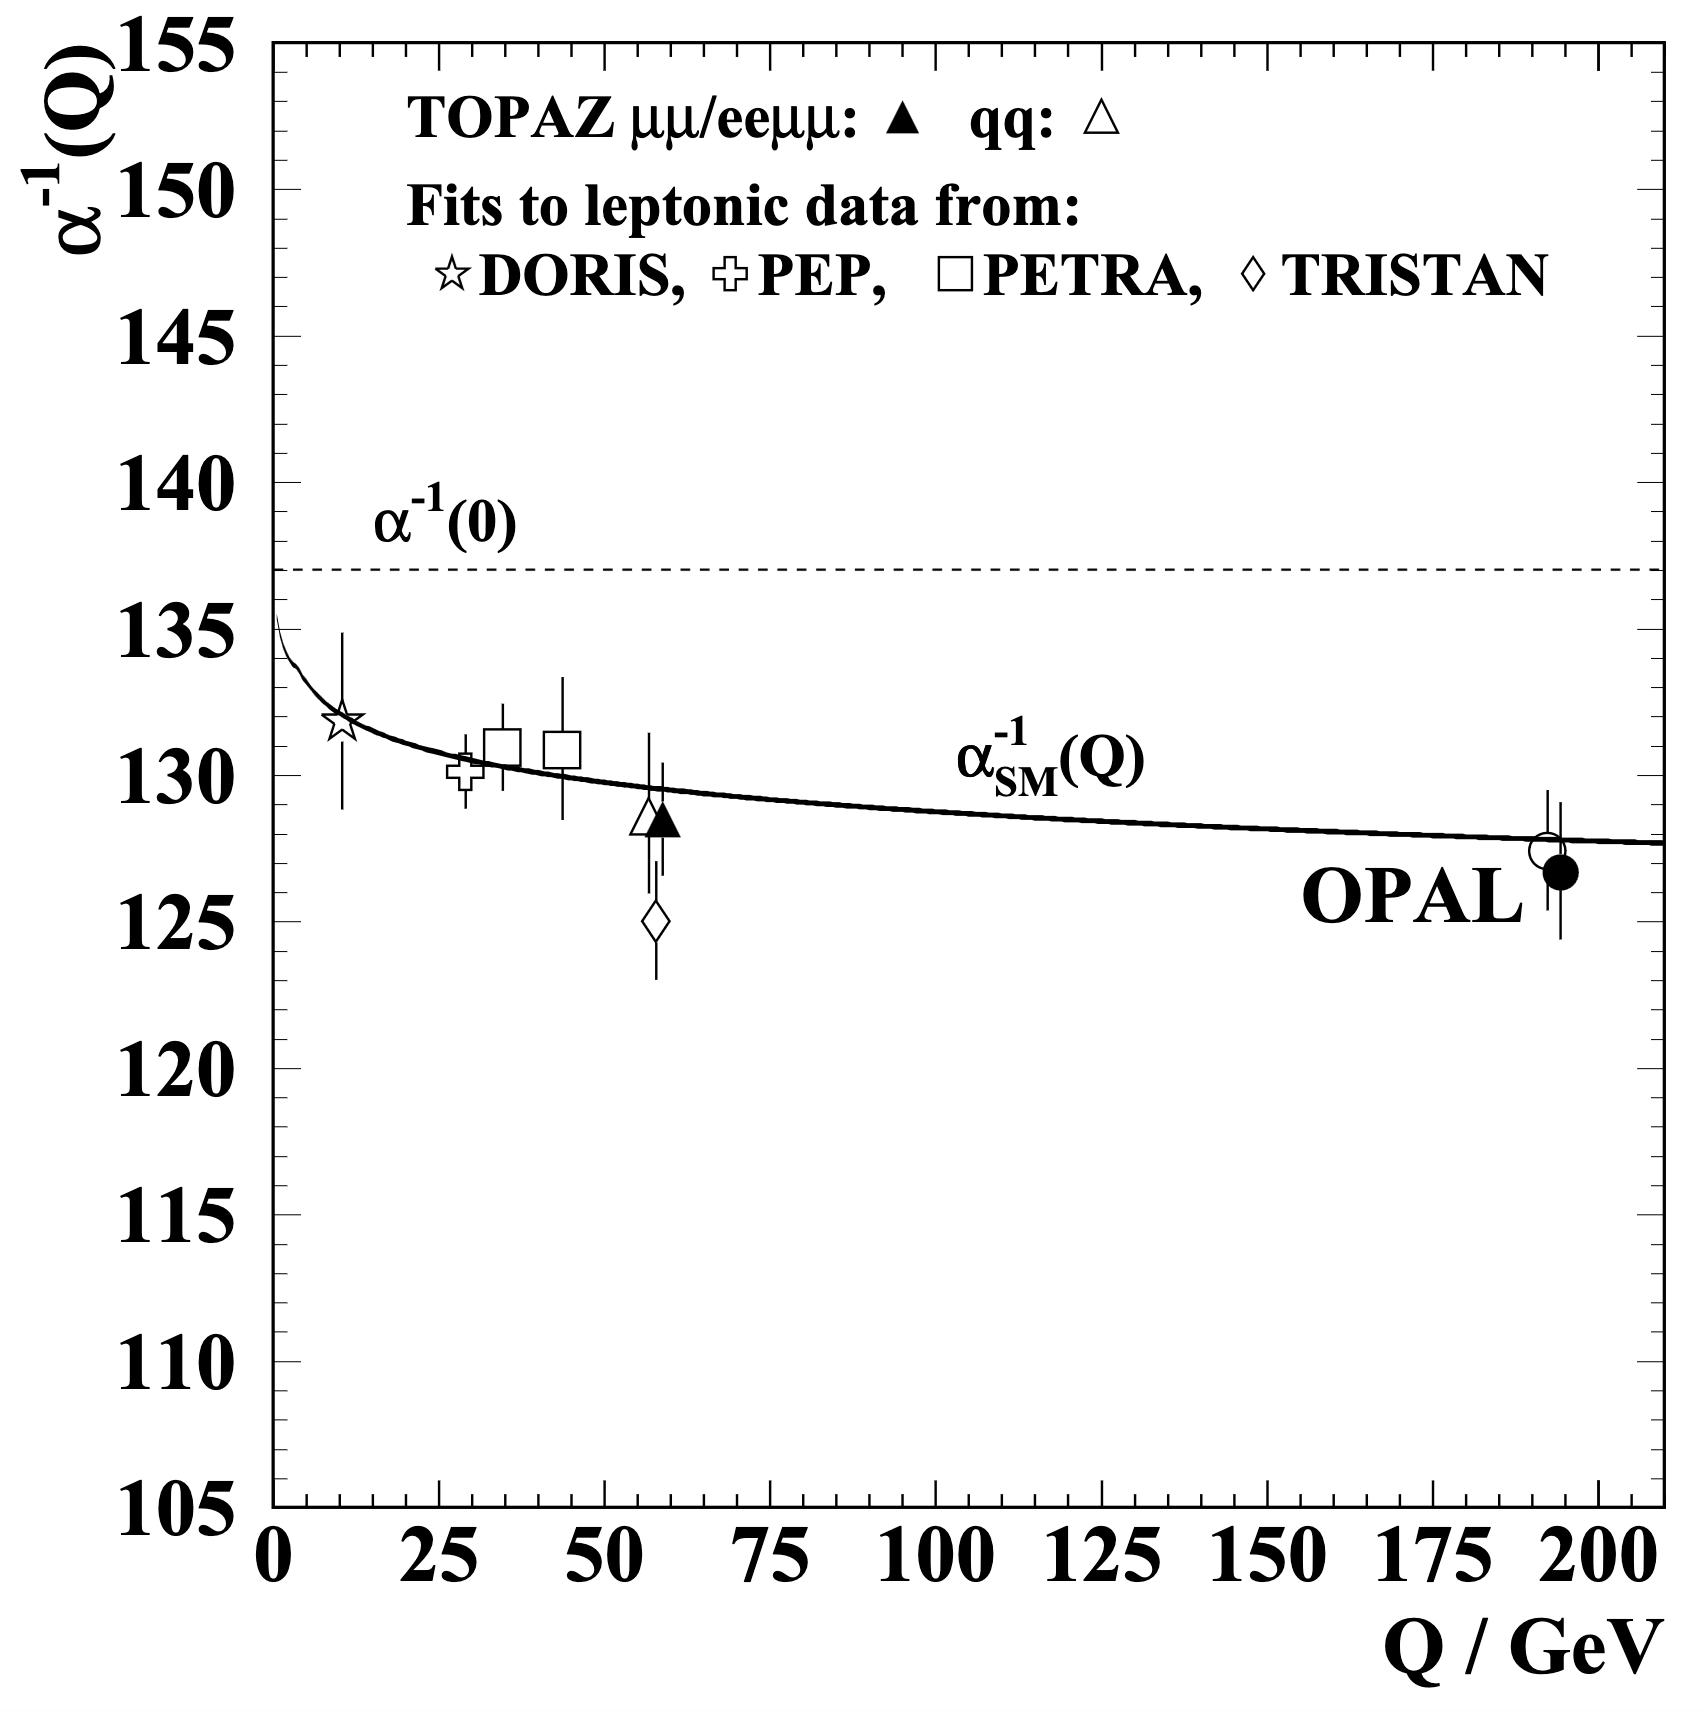
\includegraphics[width=.47\textwidth]{qed_scaling_experiment}}\hspace{5mm}
    \subfigure[]{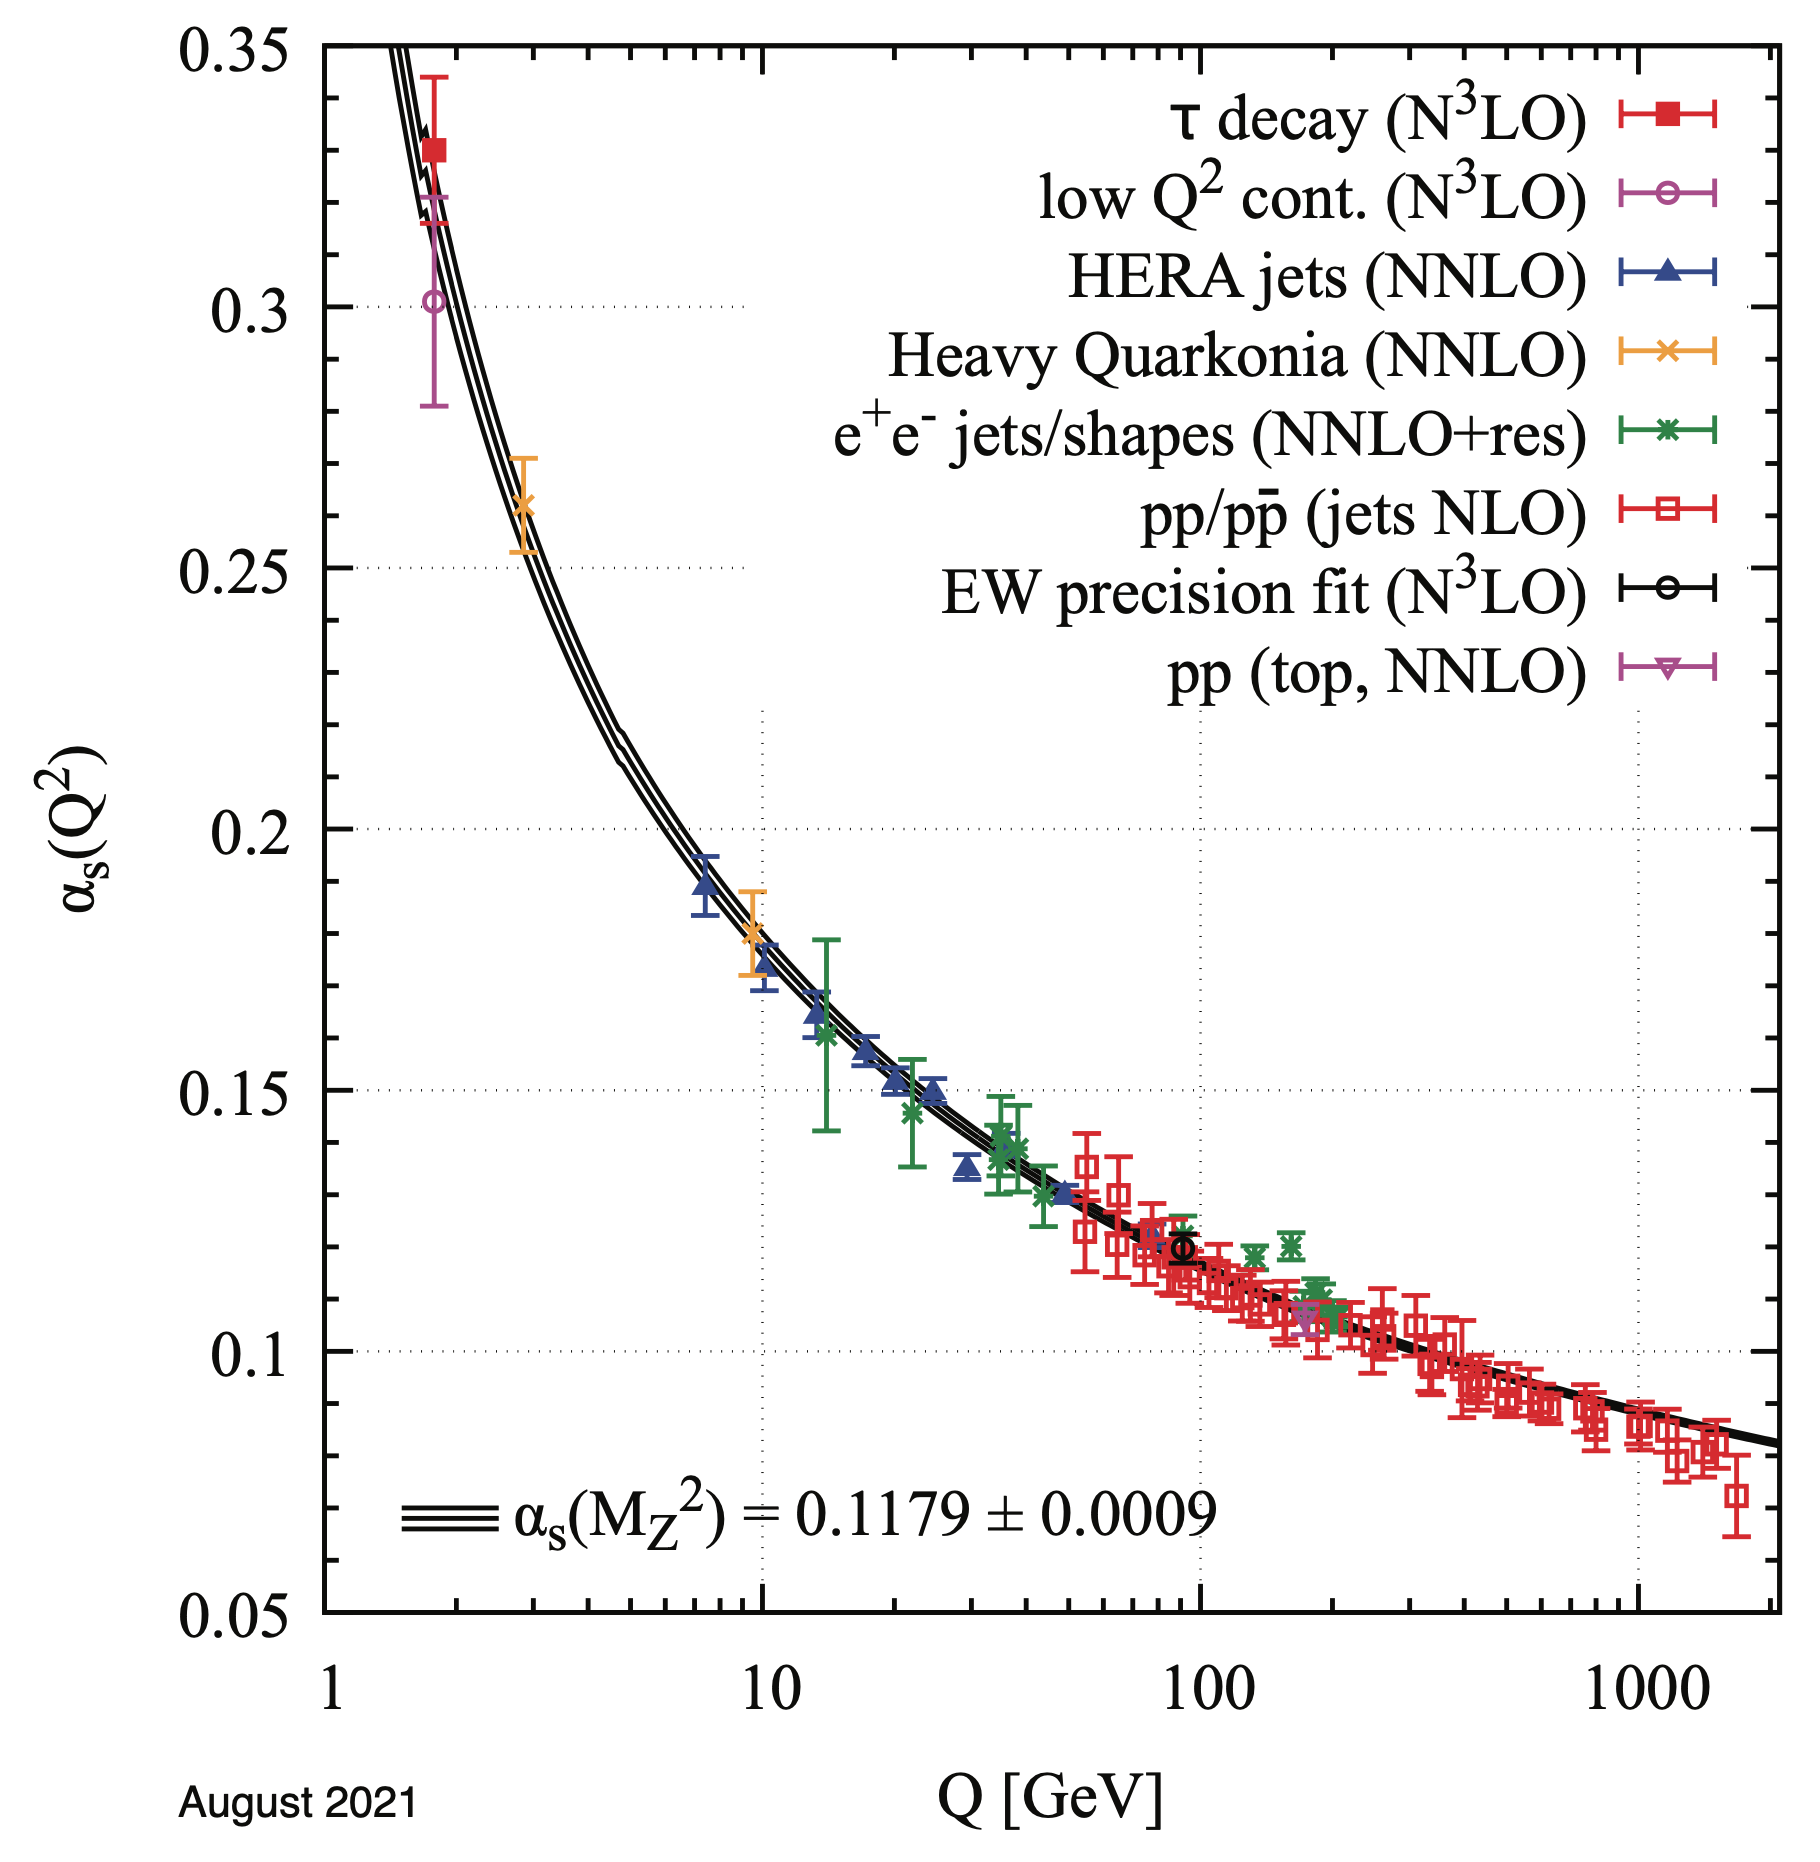
\includegraphics[width=.47\textwidth]{qcd_scaling_experiment}}
    \caption[]{Measurements of the running couplings for (\textbf{a}) \ac{qed} (note the inverted coupling on the y-axis) adopted from \citep{opal2004tests} and (\textbf{b}) \ac{qcd} adopted from \citep{particle2022review}.}
    \label{fig:renorm_scaling_exp}
\end{figure}
Most importantly the running coupling of \ac{qed} does not disturb the perturbation ansatz sketched out in section \ref{sec:qft} since $\alpha\ll1$. This is not the case for \ac{qcd} where $\alpha_S$ at $q\approx\SI{1}{GeV}$ is of $\mathcal{O}(1)$ and perturbation theory breaks down for calculations on bound hadronic states and latter processes in hadronization. While perturbation theory for \ac{qcd} remains valid for $\alpha_S\approx 0.1$ which corresponds to $q\approx \SI{100}{GeV}$ in basically all processes that are of interest at the \ac{lhc} higher order corrections must be considered in QCD calculations.

The behavior of the running coupling in \ac{qcd} is called asymptotic freedom, since the theory is free of asymptotics with increasing energy scale or decreasing distance. In turn, since the coupling increases with larger distances, this leads to color confinement, which means that colored particles can only be observed in bound states.

\section{Electroweak Unification}
The weak force can be added to the gauge invariant formalism with a $SU(2)$ symmetry and can be combined with the electromagnetic force so that both forces originate from one electroweak force by requiring a symmetry $SU(2)_L \otimes U(1)_Y$. The weak force couples to left handed chiral particle states only, e.g. for some fermion $\psi_L$. Fermions can be grouped by their characteristics into left handed doublets
\begin{equation}
    \begin{pmatrix}
        \nu_e \\ e
    \end{pmatrix}_L, \;
    \begin{pmatrix}
        \nu_\mu \\ \mu
    \end{pmatrix}_L, \;
    \begin{pmatrix}
        \nu_\tau \\ \tau
    \end{pmatrix}_L, \;
    \begin{pmatrix}
        u \\ d
    \end{pmatrix}_L, \;
    \begin{pmatrix}
        c \\ s
    \end{pmatrix}_L, \;
    \begin{pmatrix}
        t \\ b
    \end{pmatrix}_L, \;
    \label{eq:weak_doublets}
\end{equation}
with weak isospin $I=1/2$, with the third component $I_3=\pm1/2$ for the upper and lower doublet particle respectively, whereas the weak hypercharge $Y$ is associated to right handed singlets
\begin{equation}
    e_R    ,\quad \mu_R ,\quad    \tau_R ,\quad    u_R,\quad d_R ,\quad    c_R ,\quad s_R ,\quad    t_R ,\quad b_R,
\end{equation}
with $I=0$. The relation between the electric charge of the particle and these quantum numbers is governed by the Gell-Mann-Nishijima Formula $Q=I_3+Y/2$. The electroweak Lagrangian
\begin{equation}
    \mathcal{L}_\mathrm{EW} = \mathcal{L}_\mathrm{fermions}+\mathcal{L}_\mathrm{gauge}+\mathcal{L}_\mathrm{Higgs}+\mathcal{L}_\mathrm{Yukawa},
    \label{eq:L_EW}
\end{equation}
is then composed of four basic terms. Following the same steps as for \ac{qcd} and \ac{qed} the Lagrangian can be rendered gauge invariant by introducing a covariant derivative and gauge fields that are dictated by the group symmetry.

$SU(2)$ is generated through the three Pauli matrices $\bm{\sigma}$ requiring 3 vector gauge fields $W^a_\mu$, $a=\{1,2,3\}$ whereas the $U(1)$ symmetry of the vector gauge field $B_\mu$ is generated by the hypercharge $Y$. As before in order for the Lagrangian to be locally gauge invariant the new vector fields are massless. This gives the fermionic and gauge parts of the Lagrangian and will be explained below. The masses for the fermions and bosons can be incorporated via the Higgs mechanism that is described in section \ref{sec:higgs_mechanism} yielding the Higgs and Yukawa parts of the Lagrangian.


\subsubsection*{Fermion term}
To distinguish left- and right handed particle states the according spinors can be written as
\begin{equation}
    \psi_L=\frac{1-\gamma^5}{2}\psi, \quad \psi_R=\frac{1+\gamma^5}{2}\psi.
\end{equation}
These are not helicity eigenstates but rather $\psi_{L,R}$ become $\psi$, if $\psi$ has the corresponding helicity and vanish otherwise. The aforementioned doublets and singlets are then represented by
\begin{equation}
    \psi_L^j=
    \begin{pmatrix}
        \psi_{L+}^j \\ \psi_{L-}^j
    \end{pmatrix},
    \quad \psi_{R\xi}^j,
\end{equation}
with $j$ running over the doublets from equation \ref{eq:weak_doublets} and $\xi=+$ for u-type fermions and $\xi=-$ for d-type fermions.
The covariant derivative is
\begin{align}
    D_\mu^L & =\partial_\mu- i g_2 \frac{{\sigma}_a}{2}W_\mu^a+i g_1\frac{Y}{2}B_\mu, \label{eq:cov_diff_L} \\
    D_\mu^R & =\partial_\mu+ i g_1\frac{Y}{2}B_\mu,
\end{align}
with coupling $g_2$ and $g_1$ to the vector fields and $\sigma_a$ for the corresponding Pauli matrix, so that the fermionic part of the Lagrangian becomes
\begin{equation}
    \mathcal {L}_\text{fermions} = \sum_j\overline{\psi}^j_L i \gamma^\mu D_\mu^L\psi_L^j+\sum_{j,\xi}\overline{\psi}^j_{R\xi} i \gamma^\mu D_\mu^R\psi_{R\xi}^j.
    \label{eq:L_fermion}
\end{equation}

\subsubsection*{Gauge term}
The gauge field self interaction terms are
\begin{align}
    W_{\mu\nu}^a & =\partial_\mu W_\nu^a-\partial_\nu W_\mu^a+g_2\epsilon_{abc}W_\mu^b W_\nu^c, \\
    B_{\mu\nu}   & =\partial_\mu B_\nu-\partial_\nu B_\mu,
\end{align}
with $g_2$ the weak coupling constant and $\epsilon_{abc}$ the totally asymmetric Levi-Civita tensor yielding the gauge field part of the Lagrangian
\begin{equation}
    \mathcal {L}_\text{gauge} = -\frac{1}{4} W_{\mu\nu}^a W^{\mu\nu,a} - \frac{1}{4}B_{\mu\nu}B^{\mu\nu}.
\end{equation}
At this point the gauge fields $W^a_\mu$ are still massless because they would break the gauge symmetry. Masses can be incorporated into the Lagrangian with the Higgs mechanism explained in section \ref{sec:higgs_mechanism}.

\section{Higgs mechanism}\label{sec:higgs_mechanism}

In the previous sections, it was shown that the principle of local gauge invariance applied to the free Dirac Lagrangian can generate all the dynamics for a given interaction. However, this assumes that the accompanying gauge boson vector fields are massless, which is not the case for the weak interactions. The Higgs mechanism adds a field to the Lagrangian that provides mass terms for the vector bosons and fermions while preserving the principle of local gauge invariance. A way to achieve this is to introduce a complex scalar field
\begin{equation}
    \phi (x)=\frac{1}{\sqrt{2}}(\phi_1(x)+i\phi_2(x))
\end{equation}
so that a Lagrangian with a kinetic term $T(\phi)$ and a potential $V(\phi)$ with parameters $\mu$ and $\lambda$ can be constructed as
\begin{equation}
    \mathcal{L}=T(\phi)-V(\phi)=
    \left[\left(\partial_\mu\phi\right)^* (\partial^\mu\phi)\right]
    -\left[
        -\mu^2(\phi^*\phi)+\lambda(\phi^*\phi)^2
        \right].
\end{equation}
To make this Lagrangian locally gauge invariant the transformation steps from section \ref{sec:qed} on \ac{qed} can be followed. Again by replacing the derivative with the covariant derivative with some vector field $B_\mu$ and coupling $g$
\begin{equation}
    \partial_\mu \rightarrow D_\mu = \partial_\mu + ig B_\mu.
\end{equation}
The resulting Lagrangian can be made locally gauge invariant with the transformations
\begin{align}
    \phi(x)  & \rightarrow  e^{-i \alpha(x)}\phi(x), \label{eq:scalar_local_gauge} \\
    B_\mu(x) & \xrightarrow{} B_\mu(x) -\partial_\mu\alpha(x).
\end{align}
The lowest energy state of a free field theory is the vacuum state and therefore its eigenvalue $v$ is also called \ac{vev}. It is the one that minimizes the potential $V(\phi)$
\begin{equation}
    v =
    \begin{cases}
        0                                                     & \lambda>0, \mu^2<0 \\
        \sqrt{\phi_1^2+\phi_2^2}=\sqrt{\frac{\mu^2}{\lambda}} & \lambda>0, \mu^2>0,
    \end{cases}
\end{equation}
and is either 0 or forms an infinite set of minima as illustrated in figure \ref{fig:higgs_potential} by the dashed circle.
\begin{figure}
    \centering
    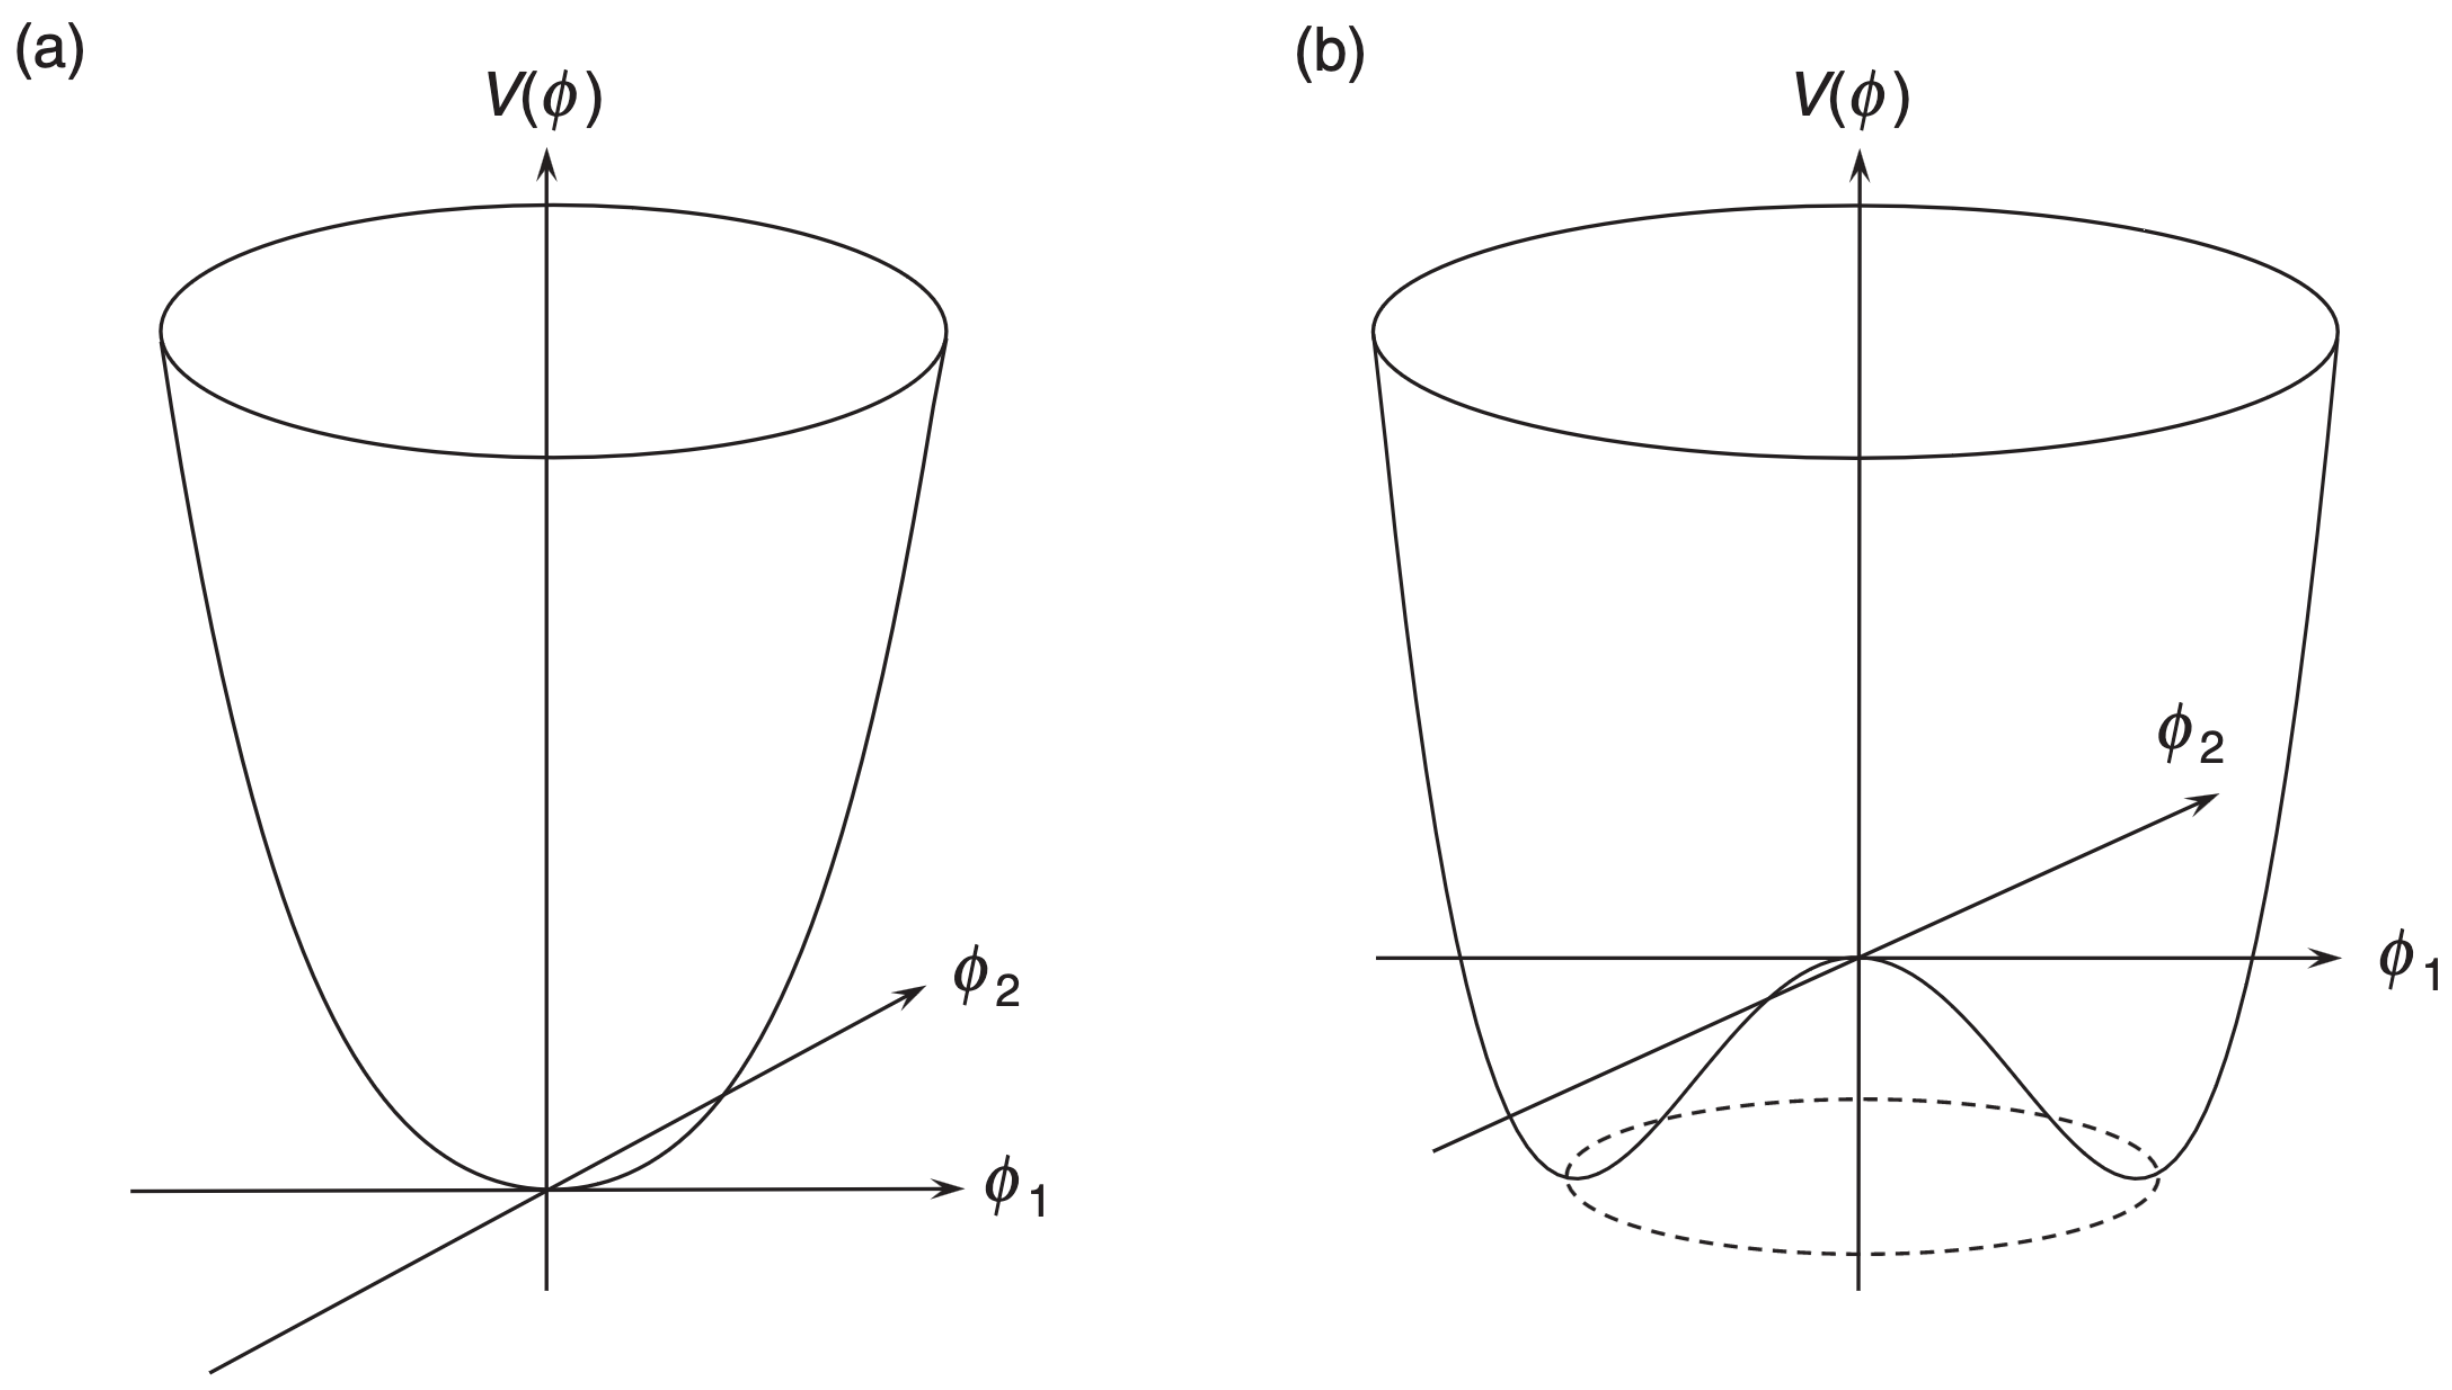
\includegraphics[width=.8\textwidth]{higgs_potential}
    \caption[]{Potential $V(\phi)$ (a) for $\lambda>0$ and $\mu^2<0$ and (b) for values $\lambda>0$ and $\mu^2>0$. Adopted from \citep{thomson2013modern}.}
    \label{fig:higgs_potential}
\end{figure}

The perturbation ansatz sketched out in section \ref{sec:qft} considers perturbations around the ground state. Thus for the ansatz to work with the $\mu^2>0$ case new field variables $\eta(x)$ and $\xi$ can be introduced so the perturbation calculus can be applied about the ground state
\begin{equation}
    \phi_1(x)=v+\eta(x),\quad \phi_2=\xi.
\end{equation}
Tthe physical vacuum state spontaneously breaks the symmetry of the Lagrangian. Furthermore the physical predictions of the Lagrangian do not depend on the choice of the gauge it can be chosen in a way that it eliminates the field $\xi$. In particular if $\alpha(x)=-\xi(x)/(gv)$ it can make the transformation from equation \ref{eq:scalar_local_gauge} unitary $UU^\dagger=1$ when expressed to first order in the fields. Moreover $\eta(x)$ can then be reinterpreted as the physical Higgs field $h(x)$
\begin{equation}
    \phi(x)  \rightarrow  e^{-i \alpha(x)}\frac{1}{\sqrt{2}}(v+\eta(x)+i\xi(x))
    \approx
    \frac{1}{\sqrt{2}}e^{-i \frac{\xi(x)}{gv}}[v+\eta(x)]e^{i\frac{\xi(x)}{gv}}
    =
    \frac{1}{\sqrt{2}}(v+h(x)).
\end{equation}
The written out Lagrangian except for constants is then
\begin{align}
    \mathcal{L}=&
    \underbrace{\frac{1}{2}(\partial_\mu h)(\partial^\mu h)-\lambda v^2 h^2}_{\text{massive h scalar}}
    -
    \underbrace{\frac{1}{4}F_{\mu\nu}F^{\mu\nu} -\frac{1}{2}g^2v^2 B_\mu B^\mu}_{\text{massive boson}}
    \nonumber 
    \\
    &+ \underbrace{g^2vB_\mu B^\mu h+\frac{1}{2}g^2 B_\mu B^\mu h^2}_{\text{h,B interactions}}
    -
    \underbrace{\lambda v h^3 -\frac{1}{4}\lambda h^4}_{\text{h self-interactions}}
\end{align}
and describes a massive scalar particle, a massive boson, interactions between the scalar and boson and as well interactions of the scalar itself depicted in figure \ref{fig:higgs_couplings}.
\begin{figure}
    \centering
    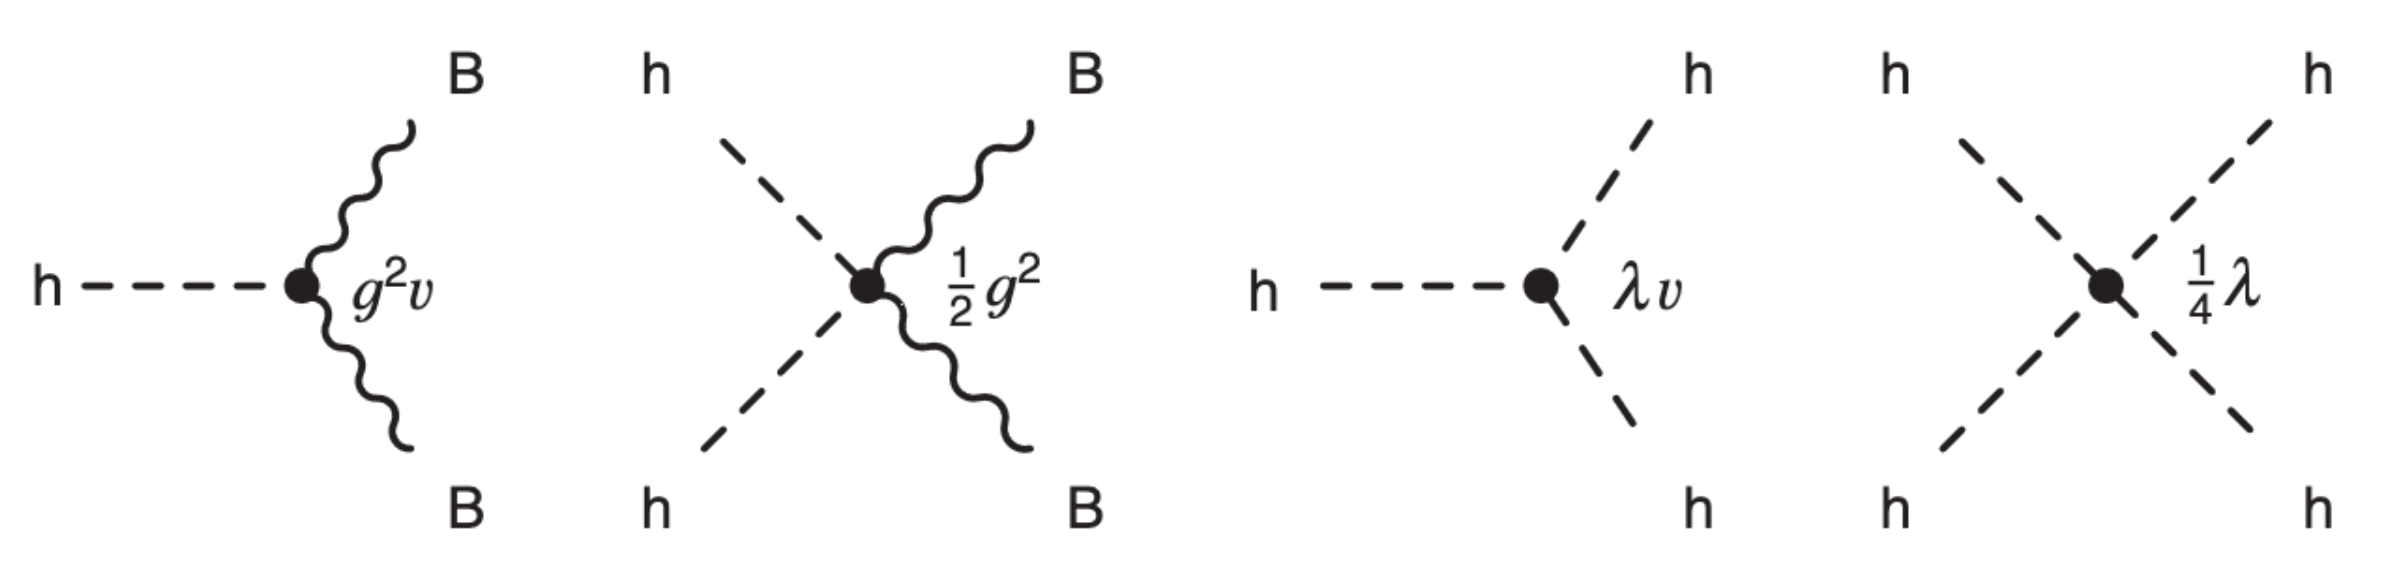
\includegraphics[width=.8\textwidth]{higgs_couplings}
    \caption[]{Higgs self interactions for a local $U(1)$ gauge symmetry. Adopted from \citep{thomson2013modern}.}
    \label{fig:higgs_couplings}
\end{figure}

\subsection*{The \ac{sm} Higgs} 
For the electroweak Lagrangian a Higgs mechanism needs to breaks down the $SU(2)_L \otimes U(1)_Y$ symmetry while maintaining the electromagnetic $U(1)_{EM}$ symmetry which is also called \ac{ewsb}. Thus the \ac{sm} Higgs field is a single isospin doublet of complex scalar fields
\begin{equation}
    \phi(x)=
    \begin{pmatrix}
        \phi^+(x) \\
        \phi^0(x)
    \end{pmatrix}
    =
    \begin{pmatrix}
        \phi_1 (x)+i \phi_2 (x) \\
        \phi_3 (x)+i \phi_4 (x),
    \end{pmatrix}
\end{equation}
with hyperchage $Y=1$ so that the covariant derivative from equation \ref{eq:cov_diff_L} reads
\begin{equation}
    D_\mu=\partial_\mu- i g_2\frac{{\sigma}_a}{2}W_\mu^a+ i\frac{g_1}{2}B_\mu.
\end{equation}

\subsubsection*{Higgs term}
The Higgs term for the electroweak Lagrangian in equation \ref{eq:L_EW} then is
\begin{equation}
    \mathcal{L}_\text{Higgs}= \left(D_\mu\phi\right)^\dagger (D^\mu\phi)-V(\phi),
    \label{eq:L_higgs}
\end{equation}
with the Higgs potential
\begin{equation}
    V(\phi) = -\mu^2\phi^\dagger\phi+\frac{\lambda}{4}\left(\phi^\dagger\phi\right)^2.
    \label{eq:Higgs_V}
\end{equation}


Since this equation was verifiable before the it was a compelling argument for the Higgs to exist.

\subsubsection*{Yukawa term}


% \section{Statistics}\label{sec:statistics}

Every scientific investigation starts with a hypothesis that is to be tested empirically. The main objective is to evaluate if the proposed hypothesis agrees or disagrees with observed data, to either accept or reject it against the null-hypothesis. The metric at hand to do so is the p-value that arises within hypothesis testing. 

In the field of high energy physics, a framework based on likelihood statistics has been developed specifically for this task. This section begins to lay out the mathematical fundamentals of the approach and explains its implementation in \textsc{pyhf} \citep{pyhf,pyhf_joss}. The following is based on \citep{cowan2011asymptotic,behnke2013data,pyhf}.
 
\subsection{Building the likelihood}\label{sec:likelihood}
The statistical model must take into account how compatible are the theoretical predictions with the observed collision events. This can be described by a likelihood $L(\bm{x} | \bm{\phi})$ which is in in general a probability for an observation $\bm{x}$ under a given set of parameters $\bm{\phi}$. Through $\bm{\phi}$ the theoretical predictions are incorporated into the probability calculation. Given that this is a counting experiment, the preferred tool of analysis are bins of a histogram $\bm{h}=(h_1,...,h_N)$.

It is useful to subdivide a measurement $\bm{x}=(\bm{n},\bm{a})$ further into observable histograms $\bm{n}$, (e.g. the invariant mass of a particle) and auxiliary measurement histograms $\bm{a}$ that help to constrain the model. Additionally, in the context of hypothesis testing it is useful to split the set of parameters $\bm{\phi}=(\bm{\psi},\bm{\Theta})$ into so-called parameters of interest $\bm{\psi}$ and nuisance parameters $\bm{\Theta}$. For this subsection it is instructive to consider only one parameter of interest, the signal strength $\mu$. 

The bin contents can then be expressed in terms of the amount of signal $s_i(\bm{\Theta})$ and background $b_i(\bm{\Theta})$ in bin $i$ that depend on the nuisance parameters. The prediction (expectation value) of the histogram bins of the observable $n_i$ can then be expressed as 
\begin{equation} \label{eq:n_i}
    \langle n_i(\mu,\bm{\Theta})\rangle = \mu s_i(\bm{\Theta}) +b_i(\bm{\Theta}). 
\end{equation}
Similarly, for auxiliary measurement bins $a_i$ their expectation value can be calculated from functions $u_i(\bm{\Theta})$ that also depend on the nuisance parameters and help to constrain the model
\begin{equation} \label{eq:a_i}
    \langle a_i(\bm{\Theta}) \rangle = u_i(\bm{\Theta}).
\end{equation}
Since this is a counting experiment in which events occur at a constant mean rate and independently of time, each bin follows a Poisson distribution
\begin{equation}\label{eq:poisson}
    \frac{r^k e^{-r}}{k!}.
\end{equation}
$r$ is the expected rate of occurrences, which translates as our prediction, whereas $k$ are the actual measured occurrences. Therefore the likelihood is a product of Poisson probabilities
\begin{equation}\label{eq:likelihood}
    L(\mu,\bm{\Theta})=
    \prod_{j=1}^N \frac{(\mu s_j(\bm{\Theta}) + b_j(\bm{\Theta}))^{n_j}}{n_j !} e^{-(\mu s_j(\bm{\Theta}) + b_j(\bm{\Theta}))}
    \prod_{k=1}^M \frac{u_k(\bm{\Theta})^{a_k}}{a_k!} e^{-u_k(\bm{\Theta})}.
\end{equation}
The last product can also be thought of penalizing the likelihood if e.g. an auxiliary measurement displays a very improbable value for a quantity. To test for a hypothesized value of $\mu$, the best choice according to the Neyman-Pearson lemma \citep{behnke2013data}, is the profile likelihood ratio that reduces the dependence to the parameter(s) of interest
\begin{equation}\label{eq:likelihood_ratio}
\lambda(\mu)=
    \frac{L(\mu,\hat{\hat{\bm{\Theta}}})}
    {L(\hat{\mu},\hat{\bm{\Theta}})}.
\end{equation}
The denominator is the unconditional maximum likelihood estimation so that $\hat{\mu}$ and $\hat{\bm{\Theta}}$ both are free to vary to maximize $L$, whereas the numerator is the found maximum likelihood conditioned on some chosen $\mu$ and the set of nuisance parameters $\hat{\hat{\bm{\Theta}}}$ that maximize the likelihood for that particular $\mu$. This definition gives $0 \leq \lambda \leq 1$. For a $\lambda \approx 1$ the hypothesized value of $\mu$ shows good agreement to the Poissonian model.

\subsection{From test statistic to p-value}
For this subsection $\mu$ can be a set of parameters of interest (defined above as $\bm{\psi}$) to be consistent with the usage in the literature. To test for alternative hypotheses it is useful to transform the profile likelihood into a test statistic $t_{\mu}$ 
\begin{equation}
    t_{\mu}=-2\log \lambda(\mu).
\end{equation}
This translates to $t_{\mu} \rightarrow 0$ as good agreement and $t_{\mu} \rightarrow \infty$ as bad agreement to the model. A right-tail p-value can then be calculated from the probability density function of $t_\mu$: \acp{pdf}$(t_\mu) = f(t_\mu \mid \mu)$
\begin{equation}\label{eq:p-value}
    p_\mu = \int_{t_{\mu ,obs}}^{\infty} 
    f(t_\mu \mid \mu) \mathrm{d}t_\mu
\end{equation}
$t_{\mu ,obs}$ is the test statistic $t_\mu$ evaluated with the observed data. This is like finding the $\mu$ for which the likelihood in the numerator of the profile likelihood ratio in equation \ref{eq:likelihood_ratio} would have the same prediction as the observation ($\mu s_j(\hat{\hat{\bm{\Theta}}}) + b_j(\hat{\hat{\bm{\Theta}}})\stackrel{!}{=}n_j$ in the likelihood of equation \ref{eq:likelihood}). Just like a probability density function for a standard normal distribution, intuitively the \acp{pdf} is how probable a particular value of the test statistic $t_\mu$ is under a fixed value of the signal strength (how often it occurs compared to all other values $t_\mu$ can have). 

This particular form is handy because there exist approximations for $f(t_\mu \mid \mu)$ \citep{cowan2011asymptotic}. Wald \citep{wald1943tests} proved that for the null hypothesis in the large sample limit, the test statistic follows a normalized sum of squared distances between the tested parameters of interest $\mu$ and its maximum likelihood estimate $\hat{\mu}$. The result was extended by Wilk \citep{wilks1938large} for any hypothesis, so the test statistic becomes
\begin{equation}
    t_\mu=\sum_i \frac{(\mu_i-\hat{\mu}_i^2)}{\sigma_i^2} + \mathcal{O}(1/\sqrt{N}).
\end{equation}
The $\hat{\mu}_i$ are in the large sample limit normally distributed with mean $\mu'$ (true values) and standard deviation $\sigma_i$. This is the definition of a non-central $\chi$-squared distribution with degrees of freedom equal to the number of parameters of interest (see section 3.1 in \citep{cowan2011asymptotic}). For one parameter of interest the distribution reads
\begin{equation}\label{eq:chi-square}
    f(t_\mu \mid \mu)=\frac{1}{2\sqrt{t_\mu}}\frac{1}{\sqrt{2\pi}}
    \left[
\exp\left(-\frac{1}{2}\left(\sqrt{t_\mu}+\sqrt{\Lambda}_\mu\right)\right)
+
\exp\left(-\frac{1}{2}\left(\sqrt{t_\mu}-\sqrt{\Lambda}_\mu\right)\right)
\right],
\end{equation}
with non-centrality parameter 
\begin{equation}
    \Lambda_\mu=\frac{(\mu-\mu')^2}{\sigma^2}.
\end{equation}
Figure \ref{fig:test_stat_example} illustrates the different steps. Being able to calculate p-values allows now to state how likely it is that the proposed hypothesis is reflected by the observed data. In other words, the p-value represents the probability, how incompatible the proposed hypothesis (prediction) is with the observation.

In the scientific community a widely accepted threshold for this is a p-value of 0.05. Though particle physicists only claim discovery of a new phenomenon for $p$ < \qty{2.87e-7}{} corresponding to 5 standard deviations of the standard normal distribution and exclude hypotheses if the p-value is not below 2 standard deviations of the standard normal distribution $p$ $\lesssim$ \qty{0.05}{}. One caveat here is that this particular form of $t_\mu$ assumes $\mu$ can also be negative, which can be non-physical depending on the impact of a new process. Test statistics and their \acp{pdf} approximations considering the different cases are covered in \citep{cowan2011asymptotic}. 
\begin{figure}
    \centering
    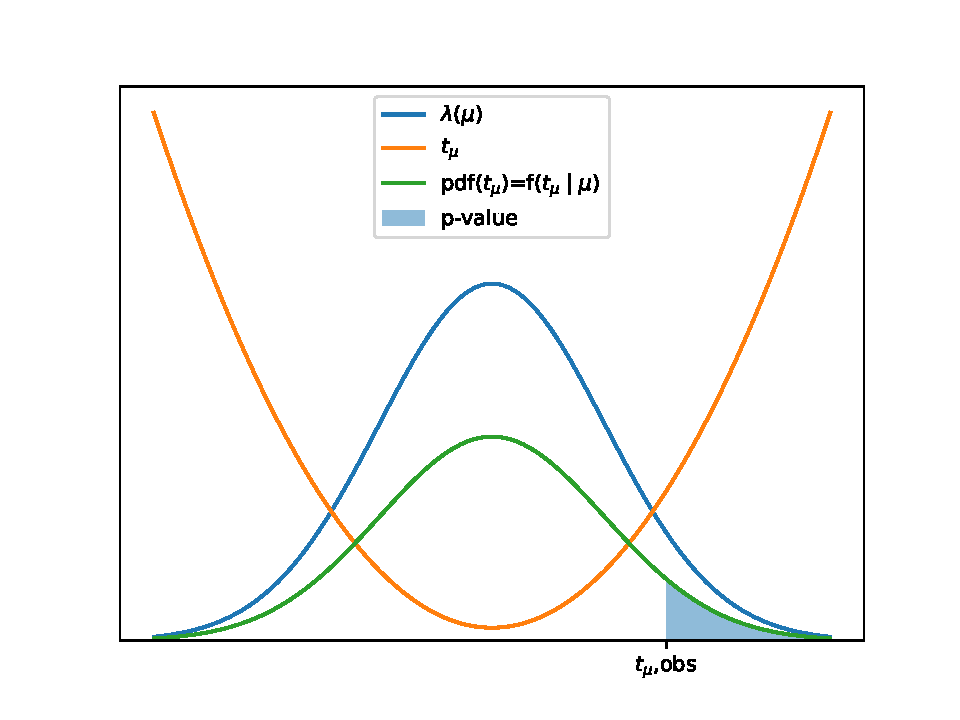
\includegraphics[width=0.8\textwidth]{test_stat_example.pdf}
        \caption[]{A sketch to follow the steps to calculate p-values. (\textbf{left}) The profile likelihood (\hexbox{1f77b4}) has essentially some hill-like form with a maximum at ${\lambda(\hat{\mu},\hat{\bm{\Theta}})}$, $t_\mu$ (\hexbox{ff7f0e}) is $-2\mathrm{ln}(\lambda)$. (\textbf{right}) For one parameter of interest in the large sample limit $f(t_\mu \mid \mu)$ follows a non-central chi-squared distribution with one degree of freedom, equation \ref{eq:chi-square}. The blue shaded area under the \acp{pdf} is a right hand sided p-value.}
    \label{fig:test_stat_example}    
\end{figure}

\subsection{The CL$_s$ value}\label{sec:cls}

Particle physicists are usually interested in two things when making statistical tests for the discovery of new phenomena: how well is the modeling of backgrounds (things we know) and whether there is evidence in the observations for a new phenomenon. This means one needs to test two hypotheses: a background only ($b$) and a signal plus background ($s+b$) hypothesis. Each will result in a p-value of their own. For example, $p_{b}=0$ would mean that the backgrounds are perfectly reflected by the observations and a $p_{s+b} < 0.05$ could be a sign of e.g. new physics. To combine these two metrics into a single score, particle physicists came up with the pseudo Confidence Level/p-value called CL$_s$ incorporating also the goodness of the modeling of the backgrounds 
\begin{equation}
    \mathrm{CL}_s=\frac{p_{s+b}}{1-p_{b}}=
    \frac
    {\int_{t_{\mu ,obs}}^{\infty} 
    f(t_{\mu,\,s+b} \mid \mu) \mathrm{d}t_\mu}
    {1-\int_{t_{\mu ,obs}}^{\infty} 
    f(t_{\mu,\,b} \mid \mu) \mathrm{d}t_\mu}.
\end{equation}
Intuitively the numerator is again just the value for the alternative hypothesis whereas the denominator penalizes CL$_s$ if the modeling of the backgrounds is not reflected in the observations. This can also be understood visually from the first figure of the paper that introduced the CL$_s$ quantity \citep{read2002presentation} (see description of fig. \ref{fig:cls}).
\begin{figure}
    \centering
    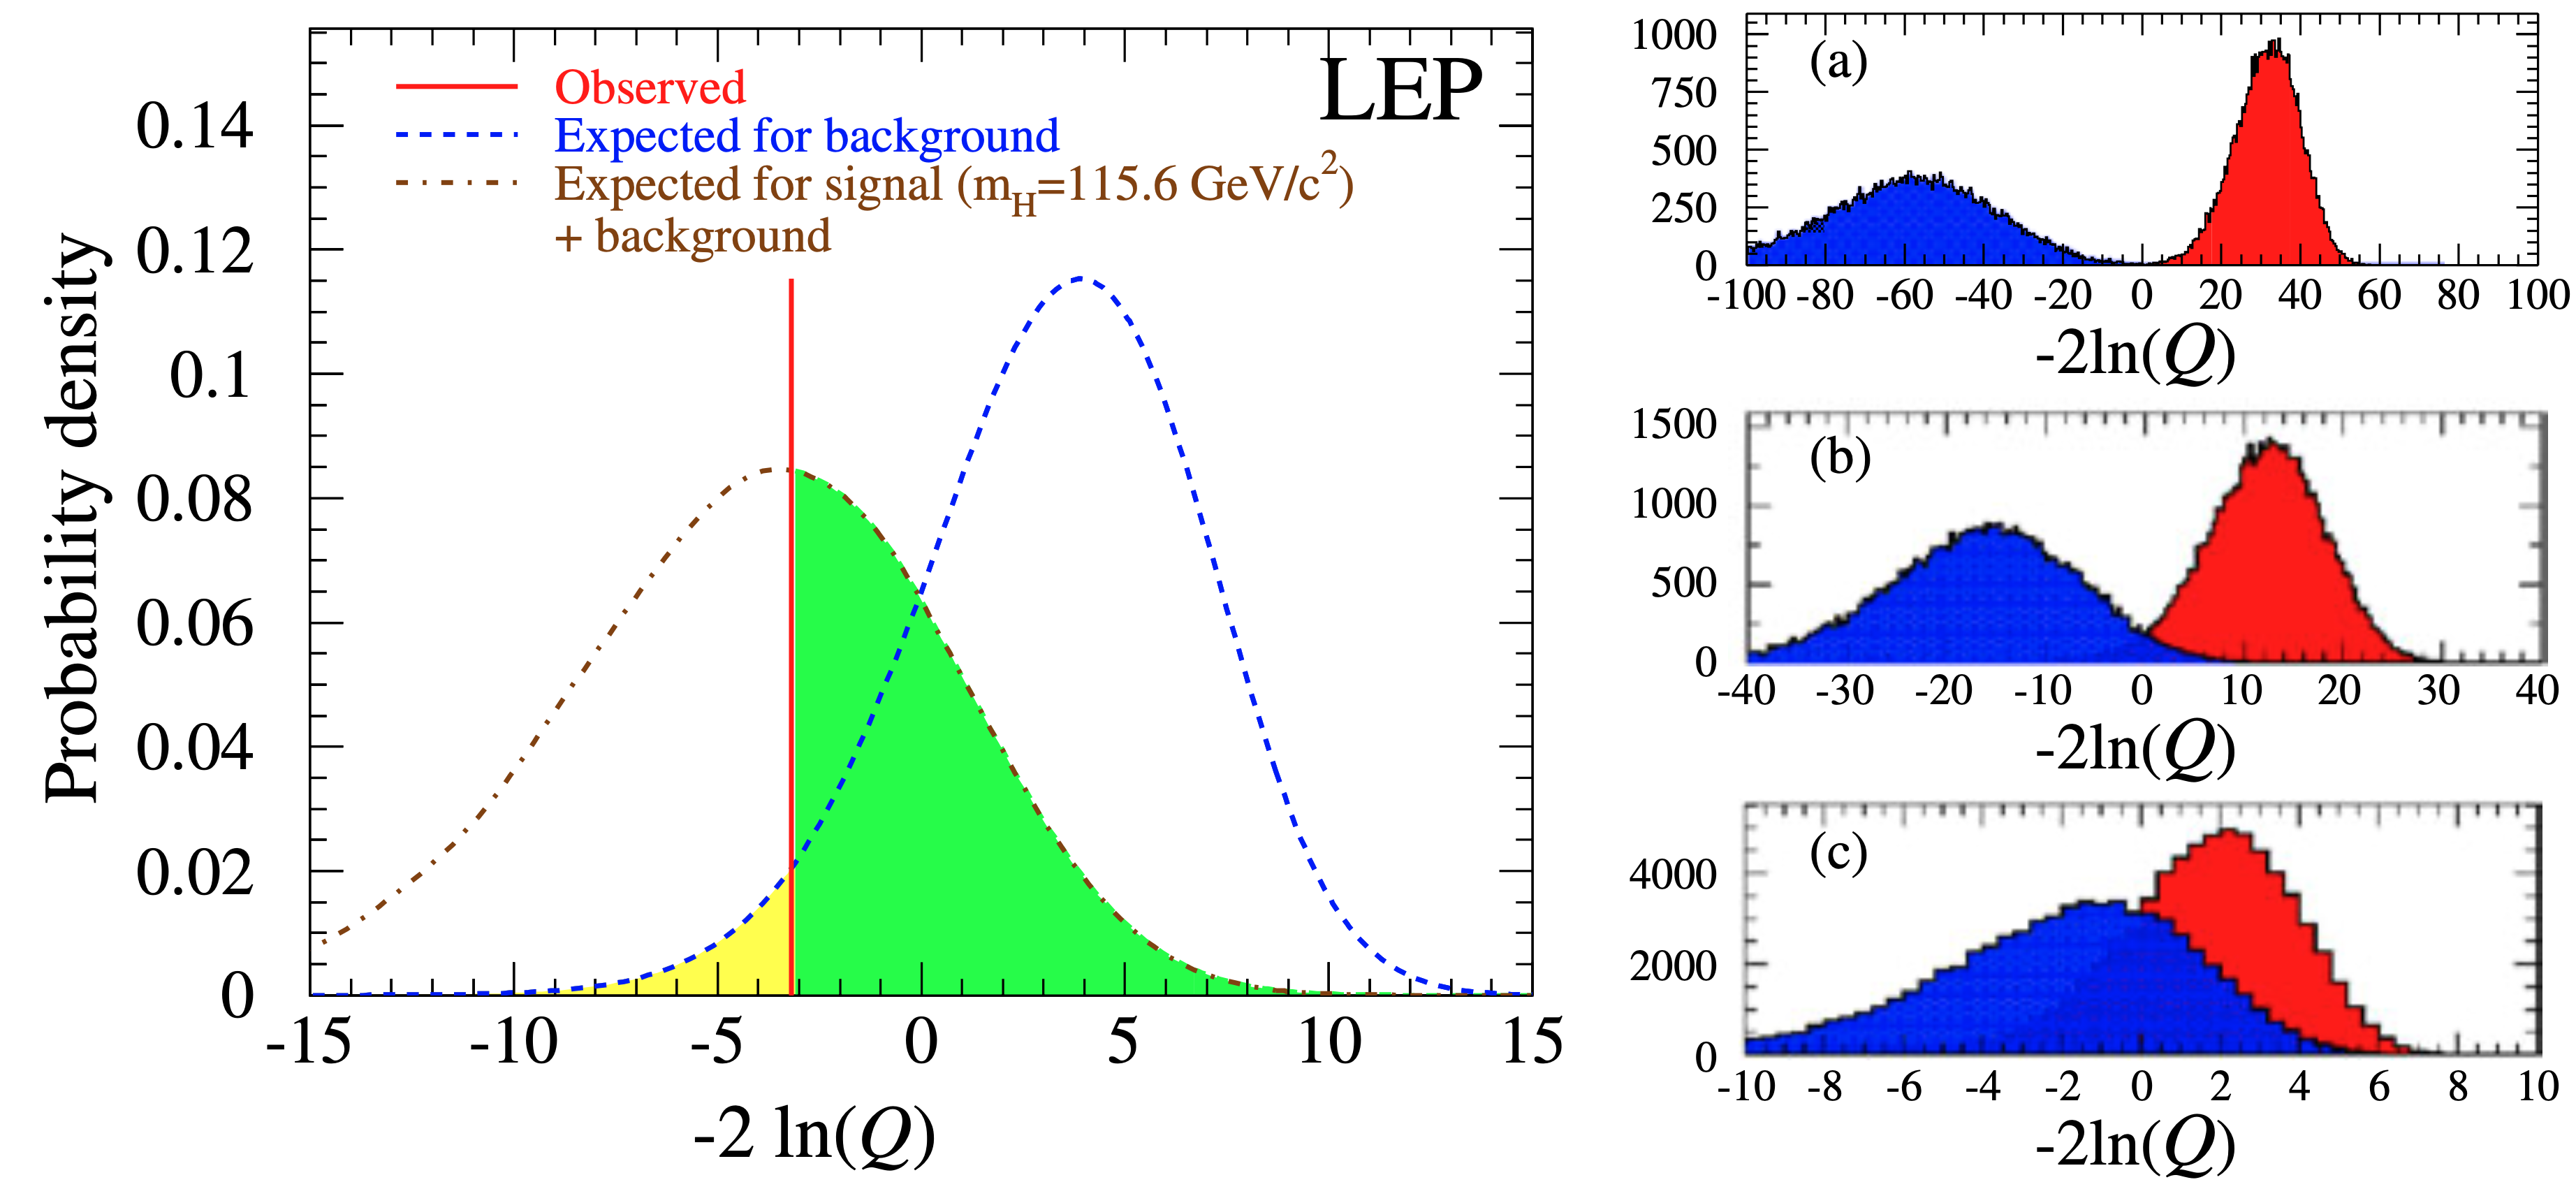
\includegraphics[width=1\textwidth]{cls.png}
        \caption[]{Probability density functions of test statistics from a Higgs search at LEP illustrating the calculation of p-values ($\lambda$ becomes $Q$). (\textbf{left}) The \acp{pdf}'s of the test statistic $f(t_\mu \mid \mu)$ of the signal + background ({\color[HTML]{804000}{$\bm{\diagup}$}}) and background ({\color[HTML]{2100FF}{$\bm{\diagup}$}}) only hypotheses. The p-value is calculated by integration from $t_{\mu,obs}$ (the red observed line ({\color[HTML]{FF0000}{$\bm{\diagup}$}})) to infinity (see eq. \ref{eq:p-value}). The green shaded area (\hexbox{00FF00}) corresponds to $p_{s+b}$ whereas the yellow area (\hexbox{FDFF02}) corresponds to $1-p_b$ since the integral over one whole \acp{pdf} is 1. (\textbf{right}) Degradation of search sensitivity from (a) to (c). Note that the colors of the \acp{pdf}'s change here to signal + background (\hexbox{2100FF}) and background only (\hexbox{FF0000}). For example putting the observation ($t_{\mu,obs}$) on the x-axis at 0 in these plots, one would get for plot (a) $p_{b}\approx 1$ and $p_{s+b}\approx 0$ resulting in a CL$_s\approx 0$, whereas with increasing overlap the CL$_s$ value increases and the sensitivity decreases.
        Taken from \citep{read2002presentation}.}
    \label{fig:cls}    
\end{figure}



\subsection{The HistFactory model}

A model used widely to build a likelihood as described in section \ref{sec:likelihood} is called HistFactory \citep{cranmer2012histfactory} and is implemented within \textsc{pyhf} \citep{pyhf}. This section is based on the introduction to the model within the documentation of \textsc{pyhf}. HistFactory reduces the building of a likelihood into a small number of basic components. For this purpose, it is again useful to think of another splitting of the model parameters $\bm{\phi}$ into

\newcommand{\freeset}{\bm{\eta}}
\newcommand{\constrset}{\bm{\chi}}
\newcommand{\singleconstr}{\chi}
\newcommand{\channelcounts}{\bm{n}}
\newcommand{\auxdata}{\bm{a}}
\newcommand{\poiset}{\bm{\psi}}
\newcommand{\nuisset}{\bm{\theta}}
\newcommand{\fullset}{\bm{\phi}}
\newcommand{\singlefull}{\phi}


\begin{equation}
 L(\bm{x}|\fullset) \quad=\quad
 L(\bm{x}|\overbrace{\poiset}^{\llap{\text{parameters of interest}}},\underbrace{\nuisset}_{\llap{\text{nuisance parameters}}}) \quad=\quad
 L(\bm{x}|\overbrace{\freeset}^{\rlap{\text{free}}},\underbrace{\constrset}_{\rlap{\text{constrained}}}) 
\end{equation}
free parameters $\freeset$ and constrained parameters $\constrset$. Free parameters are free to choose in the model and can be for example a cross-section of a process. Constrained parameters are used to incorporate uncertainties into the likelihood to constrain it. Further there might be several histograms of an observable, for example measured in orthogonal kinematic regions, that are called channels $c$. Bins have the index $b$ here and constraint terms are denoted $c_{\singleconstr}$. With that the likelihood can be described by 
\begin{equation}
L(\channelcounts, \auxdata \,|\,\freeset,\constrset) = \underbrace{\color{blue}{\prod_{c\in\mathrm{\,channels}} \prod_{b \in \mathrm{\,bins}_c}\textrm{Pois}\left(n_{cb} \,\middle|\, \nu_{cb}\left(\freeset,\constrset\right)\right)}}_{\substack{\text{Simultaneous measurement}\\%
\text{of multiple channels}}} \underbrace{\color{red}{\prod_{\singleconstr \in \constrset} c_{\singleconstr}(a_{\singleconstr} |\, \singleconstr)}}_{\substack{\text{constraint terms}\\%
\text{for }\text{auxiliary measurements}}}.
\end{equation}
The $n_{cb}$ is the observation and $\nu_{cb}(\freeset,\constrset)$ the prediction. The $c_{\singleconstr}(a_{\singleconstr} |\, \singleconstr)$ are calculated from auxiliary measurements $a_{\singleconstr}$ (the uncertainties) to constrain the parameter $\singleconstr$ and can be any function (e.g. Gaussian, Poissonian,...) the parameter/uncertainty is believed to be distributed.

The prediction is a sum of nominal bin counts\footnote{also called rates, like in the definition of a Poisson distribution} $\nu_{scb}^0$ over all samples $s$ (e.g. $t\overline{t}$, multijet-background, etc.). These nominal bin counts are subject to uncertainties. Therefore the bin counts can be varied within the bounds of these uncertainties. However the effect of this modification to the likelihood must be taken into account which is through the constraint terms. These penalize the likelihood the larger the modification to a nominal value becomes. The $\nu_{scb}^0$ are varied with multiplicative $\kappa_{scb}$ and additive modifiers $\Delta_{scb}$ 
\begin{align}
    \nu_{cb}\left(\fullset\right) &= \sum_{s\in\mathrm{\,samples}} \nu_{scb}\left(\freeset,\constrset\right)\\ &= \sum_{s\in\mathrm{\,samples}}\underbrace{\left(\prod_{\kappa\in\,\bm{\kappa}} \kappa_{scb}\left(\freeset,\constrset\right)\right)}_{\text{multiplicative modifiers}}\, \Bigg(\nu_{scb}^0\left(\freeset, \constrset\right) + \underbrace{\sum_{\Delta\in\bm{\Delta}} \Delta_{scb}\left(\freeset,\constrset\right)}_{\text{additive modifiers}}\Bigg).
\end{align}
The different types of modifiers are explained in section \ref{sec:modifiers} and the constraint terms $c_{\singleconstr}$ in section \ref{sec:constraint_terms}.

Why this is useful can be seen by considering one uncertainty to a nominal bin count estimate $\nu_{scb}^0$. By modifying $\nu_{scb}^0$ with a factor $\kappa$ in a way that increases the Poisson probability while the corresponding constraint term $c_\kappa(\kappa)$ stays around 1, it can be beneficial for the goal of maximizing the likelihood. This means the most likely/compatible value to the observed data within the modeling of the uncertainties can be found. 

\subsection{The Modifiers}\label{sec:modifiers}
In HistFactory there are by convention four types $\{\lambda,\mu,\gamma,\alpha\}$ of such multiplicative rate modifiers that are explained in this section. There are \textbf{free rate modifiers $\lambda$ and $\mu$} that affect all bins equally, like the cross-section of a process or the luminosity 
\begin{equation}
    \nu_{scb}(\mu)=\mu \nu_{scb}^0.
\end{equation}
These are bin-independent normalization factors and preserve the shape of the histogram. 
Further there are \textbf{bin-wise modifiers} $\gamma_b$ (uncorrelated shape)
\begin{equation}
    \nu_{scb}(\gamma_b)=\gamma_b \nu_{scb}^0.
\end{equation}
These are useful for example to include uncertainties of a per bin data-driven background estimate. This type without a constraint term is not of much use as if there is only one sample or channel, the fit would always match the data perfectly.
In addition there exist \textbf{interpolation parameters $\alpha$} (shape factors) that enter the modeling through an interpolation function $\eta$ instead of being the factor itself. They exist in multiplicative versions 
\begin{equation}
    \nu_{scb}(\alpha)=\eta(\alpha) \nu_{scb}^0,
\end{equation}
and additive versions
\begin{equation}
    \nu_{scb}(\alpha)=\nu_{scb}^0 + \eta(\alpha).
\end{equation}
This is useful to include systematic uncertainties. In a typical ATLAS analysis usually one knows the one standard deviation of a bin count $\eta_{-1}=\nu_{scb}^\mathrm{1down}$ and $\eta_{1}=\nu_{scb}^\mathrm{1up}$ to the nominal value $\nu_{scb}^0$ of an uncertainty. These are used to construct interpolation functions that modify the nominal value with a nuisance parameter that is also used to apply a penalization $c_\alpha$ according to the modeling of the uncertainty.

In HistFactory there exists four of such interpolation functions. For those exist an identity operator 
\begin{equation}
    \eta_0=\eta (\alpha=0) =
    \begin{cases}
        1 ,& \text{multiplicative modifier, } (\kappa) \\
        0 ,& \text{additive modifier, } (\lambda).
    \end{cases}
\end{equation}
One example of these interpolation functions that scales the bin count linearly over the known deviations $\eta_{-1}=\nu_{scb}^\mathrm{1down}$ and $\eta_{1}=\nu_{scb}^\mathrm{1up}$ is
\begin{equation}
    \eta_\mathrm{linear}(\alpha)=
    \begin{cases}
        \alpha(\eta_0 - \eta_1) ,& \alpha>0\\
        \alpha(\eta_0 - \eta_{-1}) ,& \alpha<0
    \end{cases}
\end{equation}
This is illustrated in fig. \ref{fig:interp_func}(a). For the other ones see e.g. \citep{heinrich2019searches}. It is noted that $\alpha$ is the nuisance parameter and not the function $\eta(\alpha)$ and there is an associated constraint term $c_\alpha$ to each $\alpha$.
\begin{figure}
    \centering
    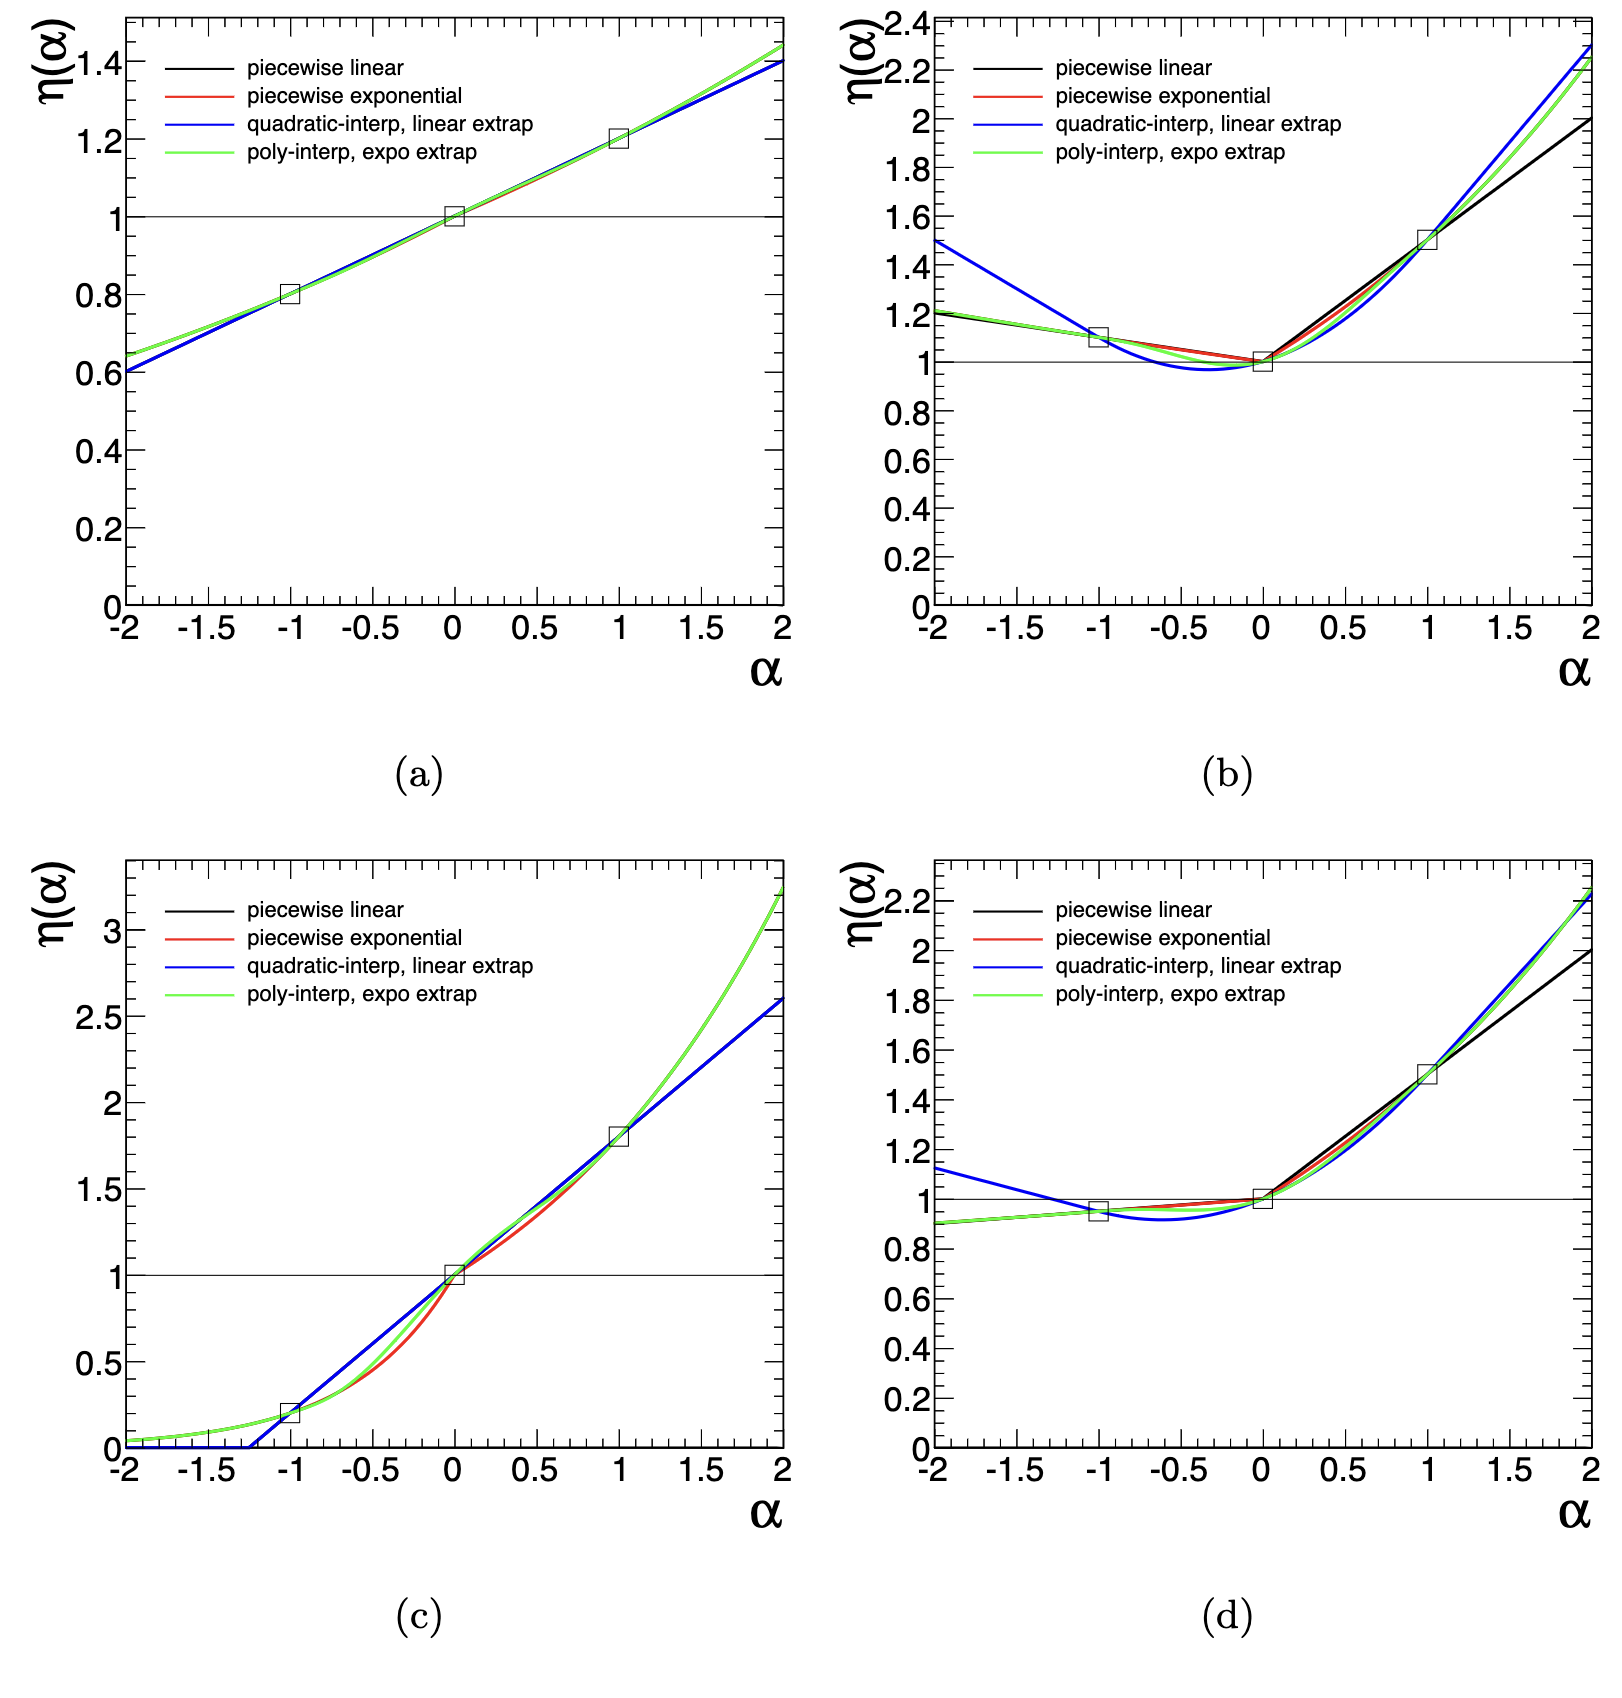
\includegraphics[width=.8\textwidth]{interp_func.png}
        \caption[]{The four interpolation functions $\eta(\alpha)$ for different up and down standard deviation values. For example in (a) the bin count will be scaled with a factor of 0.8 for an $\alpha=-1$ (1.2 for an $\alpha=1$). From \citep{cranmer2012histfactory}.}
    \label{fig:interp_func}    
\end{figure}

\subsection{The constraint terms}\label{sec:constraint_terms}
Uncertainties are modeled either Gaussian or Poissonian. The Gaussian implementation is straightforward as the uncertainty appears squared in the definition. For the interpolation function the nuisance parameter is scaled to the standard deviation values as described before $\mathrm{Gauss}(\alpha \mid a, \sigma=1)$. 

For a Poissonian constraint to a multiplicative modifier $\gamma_b$, with a nominal (most probable) value $\gamma_0=1$, the Poisson distribution must be scaled with a factor $f$, so it reflects the original bin-count uncertainty $\sigma$. To find the corresponding Poisson distribution all parameters are multiplied by a factor $f$ and is then solved for the one with the desired uncertainty. Since the variance of a Poissonian like eq. \ref{eq:poisson} is  the rate parameter $\lambda$ it follows
\begin{equation}
    \mathrm{Var}\left[\mathrm{Pois}(k=f\gamma_0,\lambda=f\gamma)\right]=\lambda\;\stackrel{\gamma=\gamma_0}{=}\;f\gamma_0=(f\sigma)^2  \quad \rightarrow \quad f=(1/\sigma^2).
\end{equation}
This completes all the requirements needed for the creation of HistFactory models. The different types of modifiers and their constraint terms are summarized in table \ref{tab:histfactory}.
\begin{table}[]
    \caption[]{Modifiers and constraint terms used in HistFactory implemented by \textsc{pyhf}. Note that the interpolation functions are called $f_p$ and $g_p$ here instead of $\eta$ as chosen in the full text. Taken from \citep{pyhf}}
    \centering
    \resizebox{0.97\textwidth}{!}{
        \begin{tabular}{l|l|l|l}\label{tab:histfactory}
            Description &Modification&Constraint Term $c_\singleconstr$ &$c_\chi$ input\\
            \hline
            Uncorrelated Shape   &$\kappa_{scb}(\gamma_b) = \gamma_b$                                                                     &$\prod_b \mathrm{Pois}\left(r_b = \sigma_b^{-2}\middle|\,\rho_b = \sigma_b^{-2}\gamma_b\right)$ &$\sigma_{b}$    \\
            Correlated Shape     &$\Delta_{scb}(\alpha) = f_p\left(\alpha\middle|\,\Delta_{scb,\alpha=-1},\Delta_{scb,\alpha = 1}\right)$ &$\displaystyle\mathrm{Gaus}\left(a = 0\middle|\,\alpha,\sigma = 1\right)$                       &$\Delta_{scb,\alpha=\pm1}$    \\
            Normalisation Unc.   &$\kappa_{scb}(\alpha) = g_p\left(\alpha\middle|\,\kappa_{scb,\alpha=-1},\kappa_{scb,\alpha=1}\right)$   &$\displaystyle\mathrm{Gaus}\left(a = 0\middle|\,\alpha,\sigma = 1\right)$                       &$\kappa_{scb,\alpha=\pm1}$    \\
            MC Stat. Uncertainty &$\kappa_{scb}(\gamma_b) = \gamma_b$                                                                     &$\prod_b \mathrm{Gaus}\left(a_{\gamma_b} = 1\middle|\,\gamma_b,\delta_b\right)$                 &$\delta_b^2 = \sum_s\delta^2_{sb}$    \\
            Luminosity           &$\kappa_{scb}(\lambda) = \lambda$                                                                       &$\displaystyle\mathrm{Gaus}\left(l = \lambda_0\middle|\,\lambda,\sigma_\lambda\right)$          &$\lambda_0,\sigma_\lambda$    \\
            Normalisation        &$\kappa_{scb}(\mu_b) = \mu_b$ & & \\
            Data-driven Shape    &$\kappa_{scb}(\gamma_b) = \gamma_b$ & & \\
        \end{tabular}
    }
\end{table}


% \chapter{The ATLAS Experiment at the LHC}

In particle physics scattering blah
In order to probe nature at the smallest scales scattering experiments are conducted as the De Broglie wavelength $\lambda=h/p$ tells that with increasing momentum smaller scales can be explored. At the moment the Large Hadron Colider at CERN (European Organization for Nuclear Research) is not only the largest machine ever built, but also the most powerful particle collider at hand .


The ATLAS detector is situated in a cavern 

\section{The Coordinate System}

\section{The Inner Detector}




\appendix
%*******************************************************
% Acronyms
%*******************************************************

\chapter{Acronyms}
\begin{acronym}[neos]
    \acro{cern}[CERN]{Organisation européenne pour la recherche nucléaire}
    \acro{atlas}[ATLAS]{A Toroidal LHC Apparatus}

    % Theory
    \acro{sm}[SM]{Standard Model}
    \acro{qft}[QFT]{Quantum Field Theory}
    \acro{qcd}[QCD]{Quantum Chromodynamics}
    \acro{qed}[QED]{Quantum Electrodynamics}
    \acro{ew}[EW]{Electroweak}
    \acro{ewsb}[EWSB]{Electroweak Symmetry Breaking}
    \acro{vev}[VEV]{Vacuum Expectation Value}
    \acro{ckm}[CKM]{Cabibbo-Kobayashi-Maskawa}
    \acro{em}[EM]{electromagnetic}
    \acro{ip}[IP]{impact parameter of tracks}
    \acro{ml}[ML]{Machine Learning}
    \acro{neos}[\textsc{neos}]{neural end-to-end-optimized summary statistics}
    \acro{hep}[HEP]{High Energy Physics}



    % Detector
    \acro{lhc}[LHC]{Large Hadron Collider}
    \acro{hllhc}[HL-LHC]{High Luminosity \acs{lhc}}
    \acro{id}[ID]{Inner Detector}
    \acro{sct}[SCT]{semiconductor tracker}
    \acro{trt}[TRT]{transition radiation tracker}
    % \acro{itk}[ITk]{Inner Tracker}
    \acro{ibl}[IBL]{insertable $b$-layer}
    % \acro{em}[EM]{electromagnetic}
    % \acro{lar}[LAr]{liquid argon}
    % \acro{ms}[MS]{muon spectrometer}
    % \acro{rpc}[RPCs]{resistive plate chambers}
    % \acro{tgc}[TGCs]{thin gap chambers}
    % \acro{mdt}[MDTs]{monitored drift tubes}
    % \acrodefplural{mdt}[MDT]{monitored drift tubes}
    % \acro{csc}[CSCs]{cathod strip chambers}
    % \acrodefplural{csc}[CSCs]{Cathod strip chambers}
    \acro{hlt}[HLT]{high level trigger}
    % \acro{roi}[RoI]{region of interest}
    % \acrodefplural{roi}[RoIs]{regions of interest}
    \acro{l1}[L1]{Level-1}
    \acro{pfo}[PFO]{Particle Flow Object}
    \acro{tcc}[TCC]{Track CaloCluster}
    \acro{ufo}[UFO]{Unified Flow Object}
    \acro{jes}[JES]{Jet Energy Scale}
    \acro{jer}[JER]{Jet Energy Resolution}
    \acro{jmr}[JMR]{Jet Mass Resolution}


    % hh4b analysis
    \acro{ggf}[GGF]{gluon-gluon fusion}
    \acro{vbf}[VBF]{vector-boson fusion}
    \acro{nnlo}[NNLO]{next-to-next-to-leading order}
    \acro{nnnlo}[N$^3$LO]{next-to-next-to-next-to-leading order}
    \acro{sr}[SR]{Signal Region}
    \acro{vr}[VR]{Validation Region}
    \acro{cr}[CR]{Control Region}
    \acro{kde}[KDE]{Kernel Density Estimation}
    \acro{bkde}[bKDE]{binned Kernel Density Estimation}

    

    % \acro{pdf}[PDF]{Parton Distribution Function}
    % \acro{dglap}[DGLAP]{Dokshitzer–Gribov–Lipatov–Altarelli–Parisi}
    \acro{mc}[MC]{Monte Carlo}
    % \acro{mpi}[MPI]{multi-parton interaction}
    % \acro{ps}[PS]{parton shower}
    % \acro{me}[ME]{matrix element}
    % \acro{isr}[ISR]{initial state radiation}
    % \acro{fsr}[FSR]{final state radiation}
    % \acro{4fs}[4FS]{four-flavour scheme}
    % \acro{5fs}[5FS]{five-flavour scheme}
    % \acro{nlo}[NLO]{next-to-leading order}
    % \acro{}[]{}

    \acro{pdf}[PDF]{Parton Density Function}


    \acro{pv}[PV]{primary vertex}
    \acro{jvt}[JVT]{jet vertex tagger}

    % \acro{ml}[ML]{Machine Learning}
    % \acro{mle}[MLE]{Maximum Likelihood Estimation}
    % \acro{llr}[LLR]{Log-likelihood ratio}
    % \acro{bdt}[BDT]{Boosted Decision Tree}
    \acro{nn}[NN]{Neural Network}
    \acro{ann}[ANN]{Artificial Neural Network}
    
    % \acro{relu}[\textsc{ReLU}]{Rectified Linear Unit}
    % \acro{adaboost}[AdaBoost]{Adaptive Boost}
    % \acro{HP}{Hyperparameter}


    % btagging
    % \acro{dl1}[DL1]{Deep Learning based heavy-flavour tagger}
    \acro{wp}[WP]{working point}
    \acro{vr}[VR]{variable radius}
    % \acro{ip}[IP]{impact parameter}
    % \acro{sv}[SV]{secondary vertex}
    % \acro{sv1}[SV1]{inclusive displaced secondary vertex reconstruction algorithm}
    % \acro{jf}[JF]{\textsc{JetFitter}}
    % \acro{smt}[SMT]{Soft Muon Tagger}
    % \acro{dips}[DIPS]{Deep Impact Parameter Sets}


    % \acro{sr}[SR]{signal region}
    % \acro{cr}[CR]{control region}
    % \acro{stxs}[STXS]{Simplified Template Cross-Section}

    % \acro{wlcg}[WLCG]{Worldwide LHC Computing Grid}
\end{acronym}

% more package info: https://www.namsu.de/Extra/pakete/Acronym.html
% Befehl	Wirkung
% ac{Kuerzel}	Bei der ersten Verwendung von ac{Kuerzel} wird die Langfassung der Abkürzung und die Abkürzung selbst in Klammern dargestellt. Wird der Befehl ac{Kuerzel} das nächste mal aufgerufen erschneit nur nocht die Abkürzung.
% \acresetall	Der Befehl \acresetall ermöglicht es das Gedächnis des ac Befehls zu löschen. Wird der Befehl \acresetall gesetzt verhält sich der ac Befehl danach wie beim ersten Aufruf (Bei allen bisher gesetzten Abkürzungen).
% acf{Kuerzel}	Mit acf{Kuerzel} gibt es ein zweites Erstes Mal für diese Abkürzung. Das heißt, sie wird wieder in der Langform und der geklammerten Abkürzung gezeigt.
% acs{Kuerzel}	acs{Kuerzel} gibt nur die Abkürzung aus.
% acl{Kuerzel}	acl{Kuerzel} gibt nur die Langform der Abkürzung aus.
% acp{Kuerzel}	Gleiche Wirkung wie ac{Kuerzel} nur hier wird der Plural ausgegeben.
% acfp{Kuerzel}	Gleiche Wirkung wie acf{Kuerzel} nur hier wird der Plural ausgegeben.
% acsp{Kuerzel}	Gleiche Wirkung wie acs{Kuerzel} nur hier wird der Plural ausgegeben.
% aclp{Kuerzel}	Gleiche Wirkung wie acl{Kuerzel} nur hier wird der Plural ausgegeben.
% acfi{Kuerzel}	Die Langform wird kursiv geschrieben, während die Abkürzung mit Kapitälchen dargestellt wird.
% iac{Kuerzel}	Hier wird der Abkürzung (beziehungsweise wenn es das erste Mal ist der Langform mit geklammerter Abkürzung) der unbestimmte englische Artikel a voran gestellt.
% Iac{Kuerzel}	Hier wird der Abkürzung (beziehungsweise wenn es das erste Mal ist der Langform mit geklammerter Abkürzung) der unbestimmte englische Artikel A voran gestellt.
% acused{Kuerzel}	Die Abkürzung wird als gesetzt markiert (gleiche Wirkung wie der ac Befehl) aber nicht angezeigt. Danach zeigt der ac Befehl nur noch die Abkürzung an.
% acsu{Kuerzel}	Zeigt die Abkürzung an und markiert sie als gesetzt.
% aclu{Kuerzel}	Zeigt die Langform an und markiert sie als gesetzt.

%-------------------------------------------------------------

    \thispagestyle{empty}
    \cleardoublepage
    
    \phantomsection
    \bibliography{bib} 
    
\cleardoublepage    
\pagestyle{schluss}
\begin{center}
    \textbf{Statutory Declaration - Eidesstattliche Erklärung}
\end{center}

I declare that I have authored this thesis independently, that I have not used other than the declared sources/ resources and that I have explicitly marked all materials which has been quoted either literally or by content form the used sources.
\par
Hiermit erkläre ich, dass ich die vorliegende Arbeit selbstständig verfasst, andere als die angegebenen Quellen/Hilfsmittel nicht benutzt und die den benutzten Quellen wörtlich und inhaltlich entnommenen Stellen als solche kenntlich gemacht habe.

\begin{flushright}
\vspace{1.5cm}
Berlin, \today
\vspace{2cm}

\makebox[5cm]{\hrulefill}

Frederic Renner
\end{flushright}


\end{document}



